\chapter{Images of the experiments}
In this appendix we present: Section \ref{appb:fig} -- pictures, that additionally illustrate the discussion from chapters on the methods, results and future work; Section \ref{appb:mobile-screenshots} -- screenshots with use of the developed mobile application, and avatars images synthesized on the mobile hardware; Section \ref{appb:exps} -- training and test images; loss and metrics plots of the performed experiments.
\section{Auxiliary illustrations}
\label{appb:fig}
\begin{figure}[!h]
	\centering
	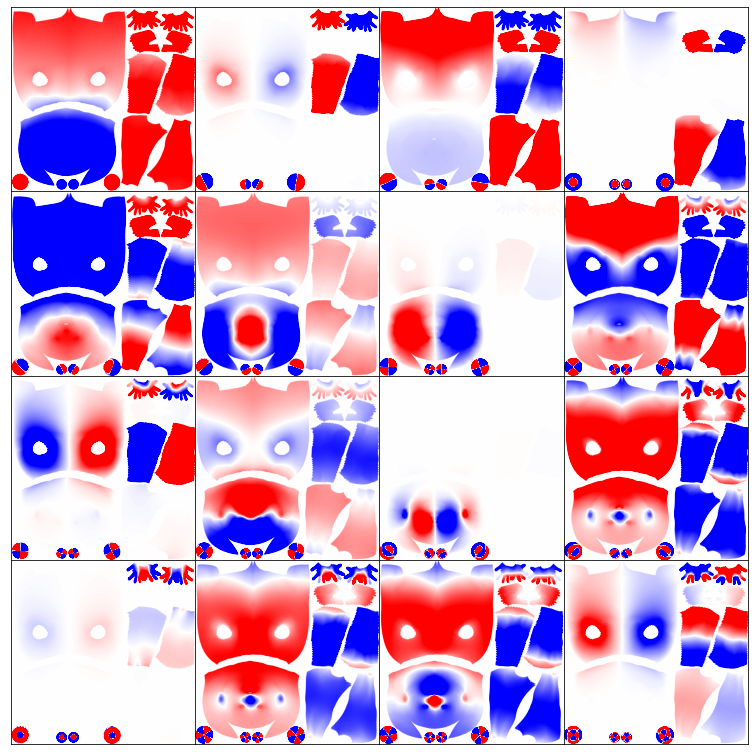
\includegraphics[height=10cm]{\imgfp/spectral_ntex}
	\caption{Baseline initialization of a neural texture with $C$ channels, containing $C$ dimensional spectral coordinates of a graph composed from mesh vertices. Notice that in different channels it distinguishes body parts, there's a channel where two legs are colored is an opposite way, similarly for arms, hands, head, upper body, etc. Compared to random initialization, it helps to convey information to the neural renderer about which body part it renders.}
	\label{fig:spectral_ntex}
\end{figure}
\begin{figure}
	\centering
	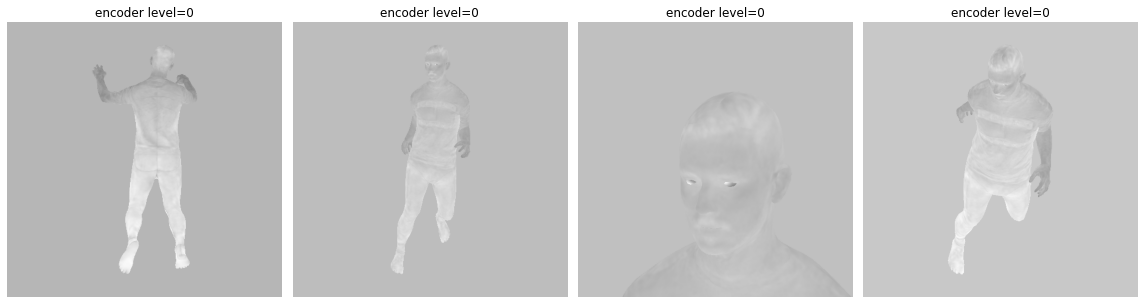
\includegraphics[width=\textwidth]{\imgfp/interm_features/03_e0}%
	\hfill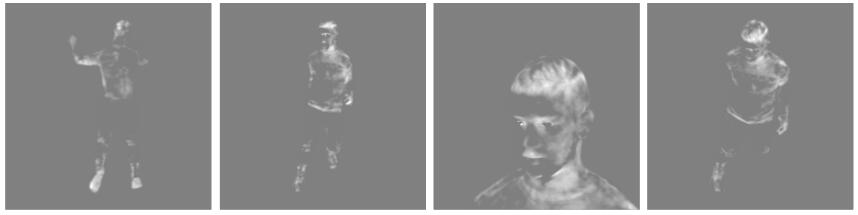
\includegraphics[width=\textwidth]{\imgfp/interm_features/03_e1}%  
	\hfill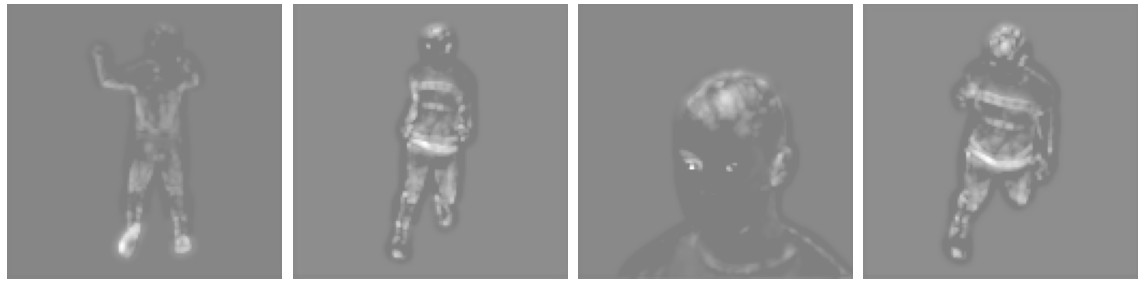
\includegraphics[width=\textwidth]{\imgfp/interm_features/03_e2}%
	\hfill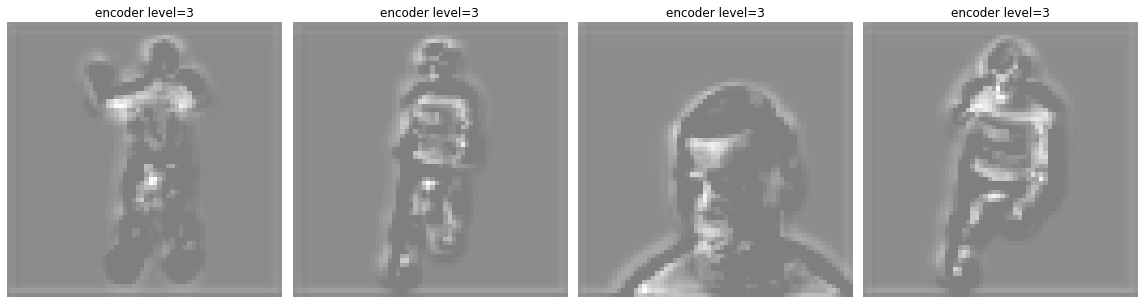
\includegraphics[width=\textwidth]{\imgfp/interm_features/03_e3}%
	\hfill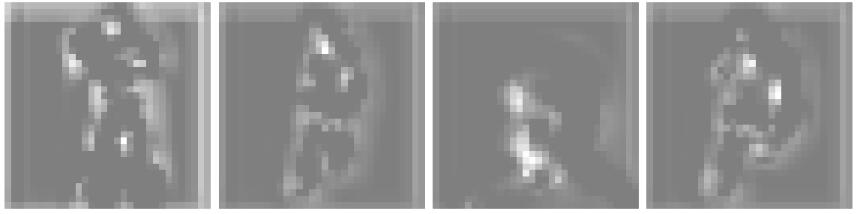
\includegraphics[width=\textwidth]{\imgfp/interm_features/03_e4}%
	\caption{One channel of activations by intermediate levels of the neural renderer's \textit{encoder}. The pipeline is plainly trained on zoomed images. Notice that the features seem activated over the whole body.}
	\label{fig:interm03_encoder}
\end{figure}
\begin{figure}
	\centering
	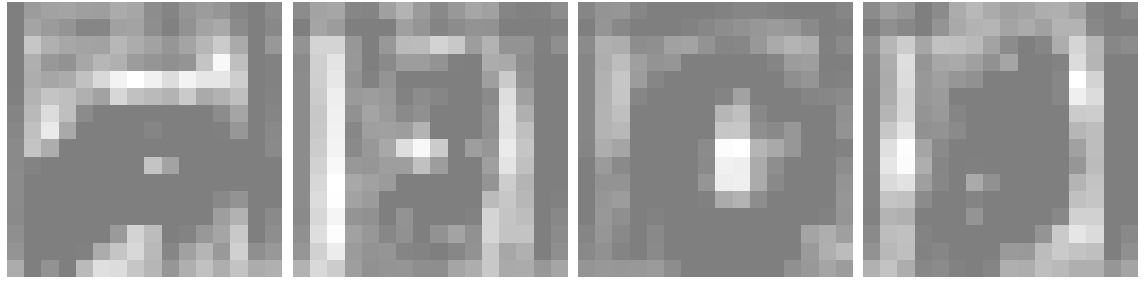
\includegraphics[width=0.9\textwidth]{\imgfp/interm_features/03_d0}%
	\hfill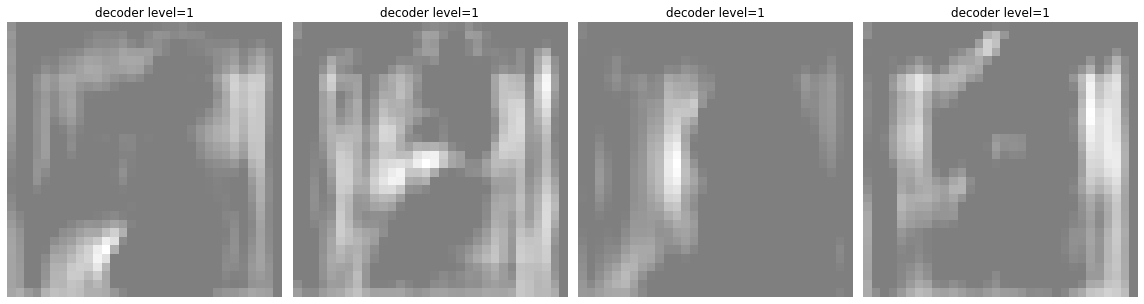
\includegraphics[width=0.9\textwidth]{\imgfp/interm_features/03_d1}%  
	\hfill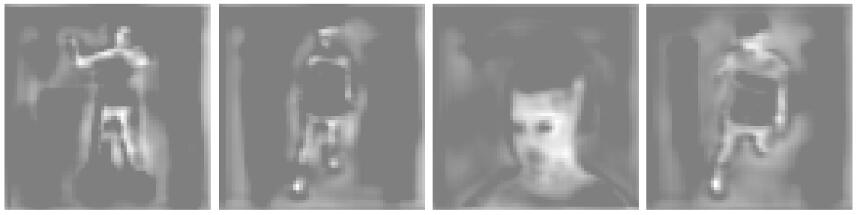
\includegraphics[width=0.9\textwidth]{\imgfp/interm_features/03_d2}%
	\hfill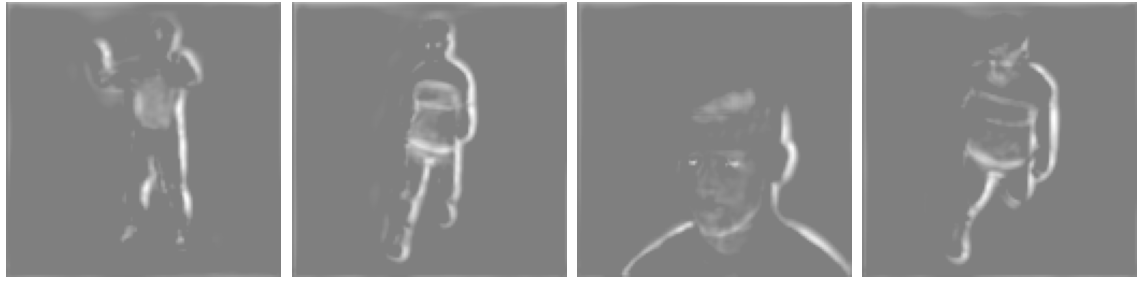
\includegraphics[width=0.9\textwidth]{\imgfp/interm_features/03_d3}%
	\hfill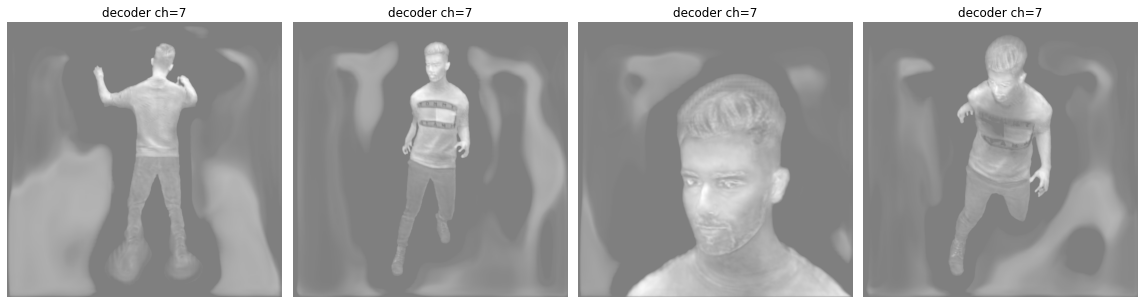
\includegraphics[width=0.9\textwidth]{\imgfp/interm_features/03_dout}%
	\hfill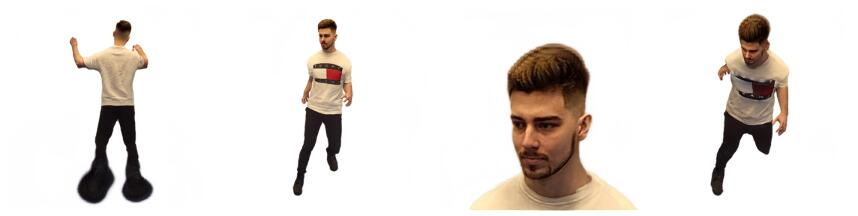
\includegraphics[width=0.9\textwidth]{\imgfp/interm_features/03_rgb}
	\caption{One channel of activations by intermediate levels of the neural renderer's \textit{decoder}. The pipeline is plainly trained on zoomed images. Notice that the space around the human image has a wavy, non-uniform structure. We speculate, that having it helps to make a more accurate segmentation in the neural renderer's heads. }
	\label{fig:interm03_decoder}
\end{figure}
\begin{figure}
	\centering
	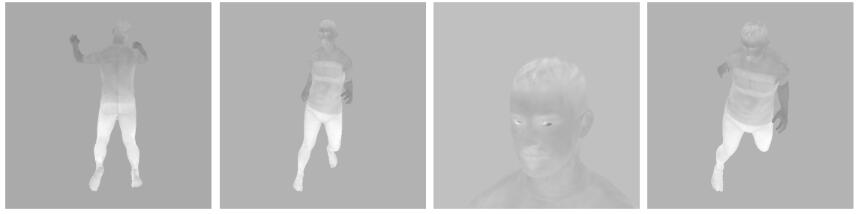
\includegraphics[width=\textwidth]{\imgfp/interm_features/bnf_e0}%
	\hfill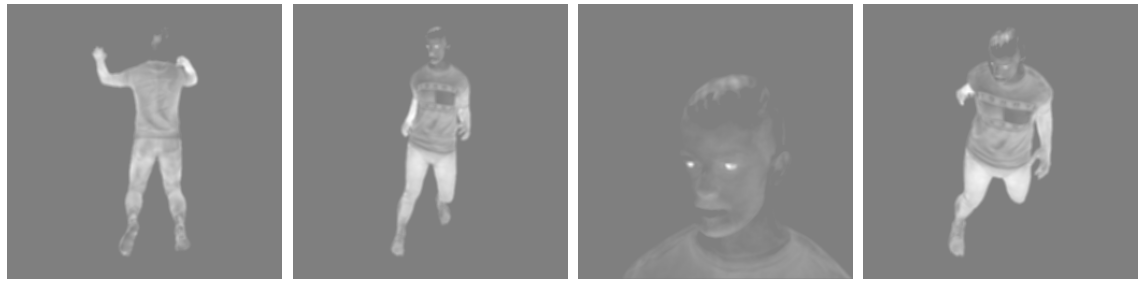
\includegraphics[width=\textwidth]{\imgfp/interm_features/bnf_e1}%  
	\hfill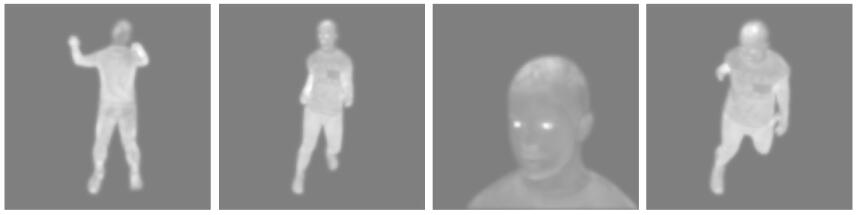
\includegraphics[width=\textwidth]{\imgfp/interm_features/bnf_e2}%
	\hfill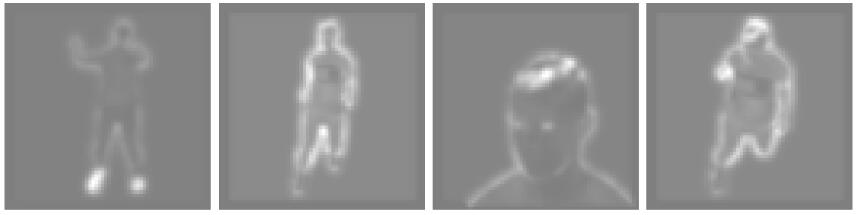
\includegraphics[width=\textwidth]{\imgfp/interm_features/bnf_e3}%
	\hfill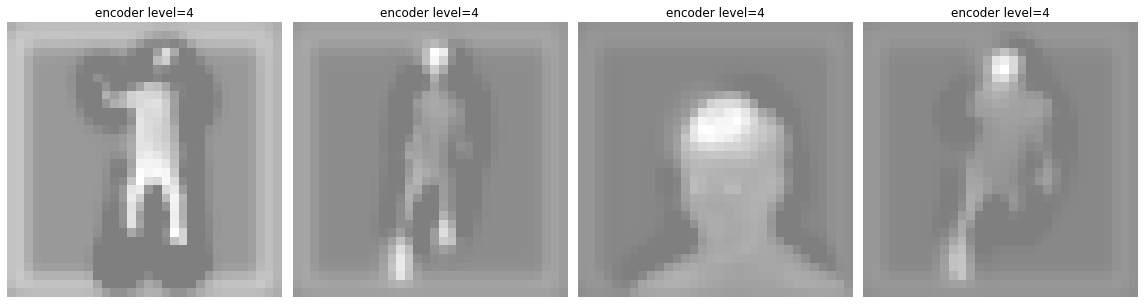
\includegraphics[width=\textwidth]{\imgfp/interm_features/bnf_e4}%
	\caption{One channel of activations by intermediate levels of the neural renderer's \textit{encoder}. The pipeline is trained on zoomed images, but Batch Normalization layers collect running statistics only on full-body images. Notice that some layers specifically trigger on unseen parts of the body that are rarely seen (bottom of boots, top of the head).}
	\label{fig:interm06_encoder}
\end{figure}
\begin{figure}
	\centering
	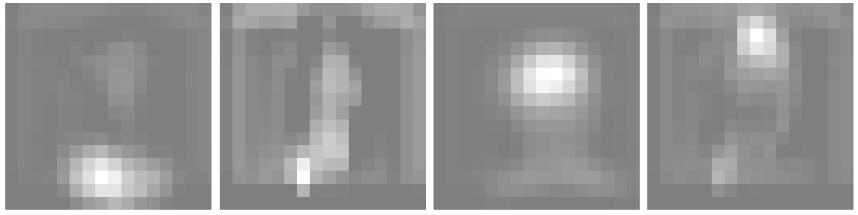
\includegraphics[width=0.9\textwidth]{\imgfp/interm_features/bnf_d0}%
	\hfill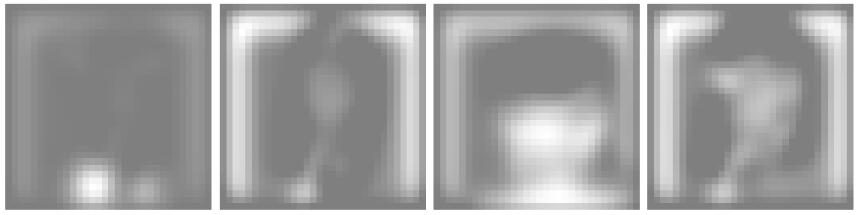
\includegraphics[width=0.9\textwidth]{\imgfp/interm_features/bnf_d1}%  
	\hfill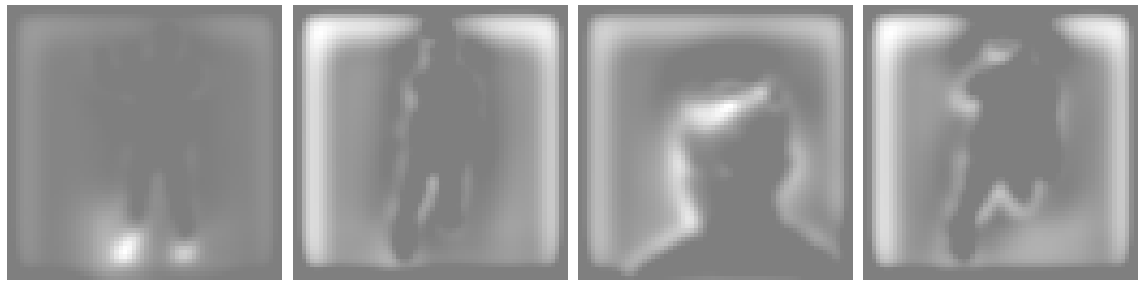
\includegraphics[width=0.9\textwidth]{\imgfp/interm_features/bnf_d2}%
	\hfill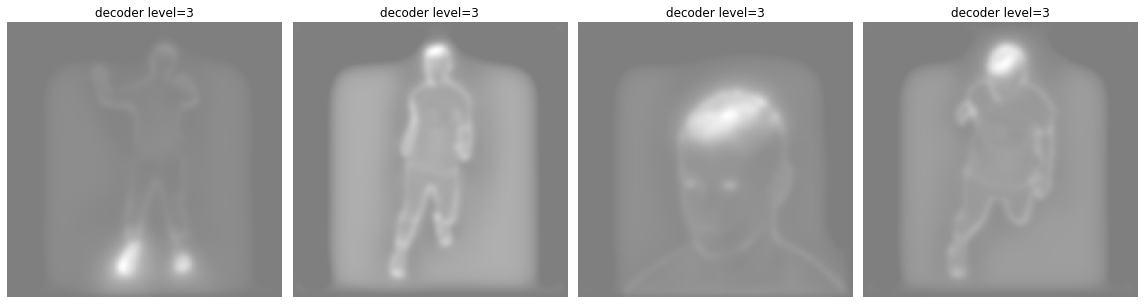
\includegraphics[width=0.9\textwidth]{\imgfp/interm_features/bnf_d3}%
	\hfill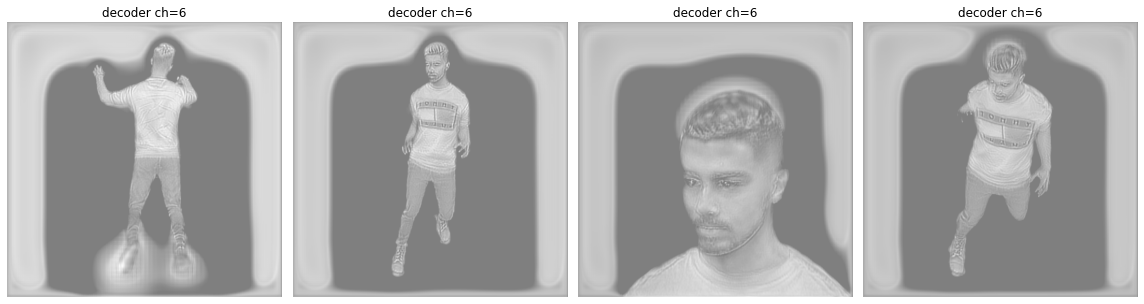
\includegraphics[width=0.9\textwidth]{\imgfp/interm_features/bnf_dout}%
	\hfill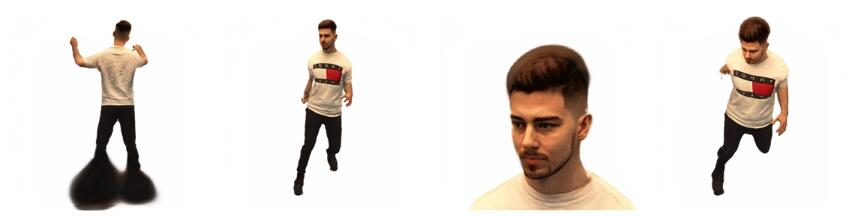
\includegraphics[width=0.9\textwidth]{\imgfp/interm_features/bnf_rgb}%
	\caption{Intermediate activattions of the neural renderer's \textit{decoder}, trained on zoomed images, but Batch Normalization layers collect running statistics only on full-body images. Notice that the space starts to form a structure that retains one value near image border, and a sharply different number around the body. We speculate, that leads to failure in segmentation, and thus the "bubble" effect around feet and the head. }
	\label{fig:interm06_decoder}
\end{figure}
\begin{figure}
	%\fboxrule=2pt
	\centering
	\begin{subfigure}[b]{0.48\textwidth}
		\centering
		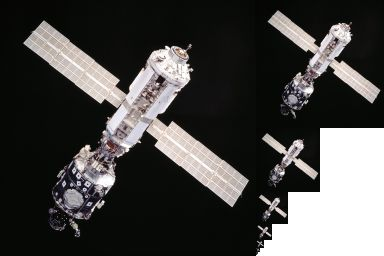
\includegraphics[height=5.5cm]{\imgfp/mips/mipmap}%
		\caption{}
		\label{fig:mipmap}
	\end{subfigure}
	\hfill
	\begin{subfigure}[b]{0.48\textwidth}
		\centering
		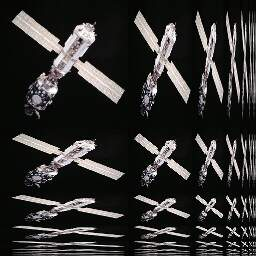
\includegraphics[height=5.5cm]{\imgfp/mips/anisotropic}
		\caption{}
		\label{fig:anisotropic}
	\end{subfigure}
	\caption{(\protect\subref{fig:mipmap}) An example collation of MIP-maps for a texture. It's repeatedly downscaled by a factor of 2, and each scale is pre-processed with an offline filtering algorithm. During rasterization, if a triangle spans a small area on the image, a particular MIP-map scale is chosed to interpolate the texture values. (\protect\subref{fig:anisotropic}) Anisotropic filtering pre-processes with additional variants for each level of downscales, that are squashed along axes. Images from \href{https://en.wikipedia.org/wiki/Anisotropic_filtering}{en.wikipedia.org/wiki/Anisotropic\_filtering}} 
\end{figure}
\begin{figure}
	\centering
	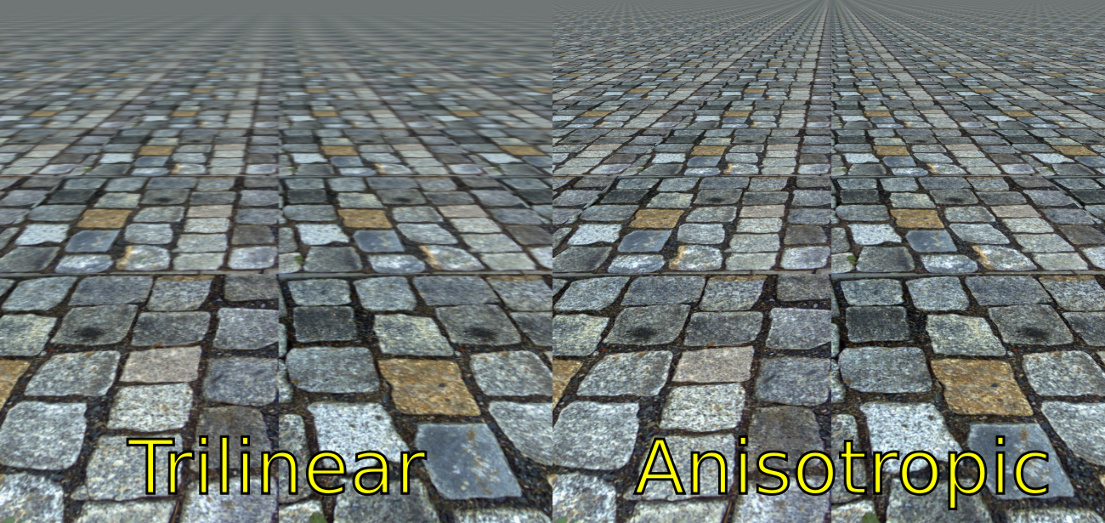
\includegraphics[height=6.5cm]{\imgfp/mips/anisotropic-result-s}
	\caption{By using anisotropically filtered scales of the texture, we could better rasterize triangles that are at steep angles to the camera. Image from \href{https://en.wikipedia.org/wiki/Anisotropic_filtering}{en.wikipedia.org/wiki/Anisotropic\_filtering}}
	\label{fig:anisotropic_result}
\end{figure}
\begin{figure}
	%\fboxrule=2pt
	\centering
	\begin{subfigure}[b]{0.49\textwidth}
		\centering
		\includegraphics[width=\linewidth]{\imgfp/mobile_inference/A01_07_nomips/000435}%
		\caption{}
		\label{fig:no_mipmap_inference}
	\end{subfigure}
	\hfill
	\begin{subfigure}[b]{0.49\textwidth}
		\centering
		\includegraphics[width=\linewidth]{\imgfp/mobile_inference/A01_07_mips_anisotropic/000435}
		\caption{}
		\label{fig:anisotropic_inference}
	\end{subfigure}
	\caption{Comparison of images synthesized on mobile, when MIP mapping with anisotropic fitering is used (\protect\subref{fig:anisotropic_inference}) or not (\protect\subref{fig:no_mipmap_inference}) for rasterization of the input. Unfortunately, the difference is negligible in our case. It can be barely seen on the edges of the mesh, where the triangles face at the most extreme angle to the camera. The processing by the neural renderer further reduces the difference.}
\end{figure}
\begin{figure}
	%\fboxrule=2pt
	\centering
	\begin{subfigure}[b]{0.35\textwidth}
		\centering
		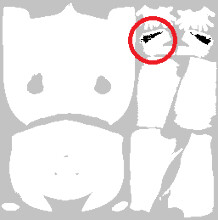
\includegraphics[width=\linewidth]{\imgfp/ntex_patch/ntex-grad}%
		\caption{}
		\label{fig:ntex-grad}
	\end{subfigure}
	\hfill
	\begin{subfigure}[b]{0.3\textwidth}
		\centering
		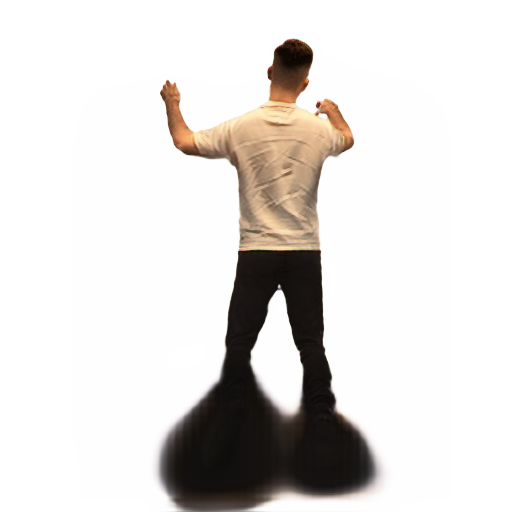
\includegraphics[width=\linewidth]{\imgfp/ntex_patch/fail}
		\caption{}
		\label{fig:ntex-artifact}
	\end{subfigure}
	\hfill
	\begin{subfigure}[b]{0.3\textwidth}
		\centering
		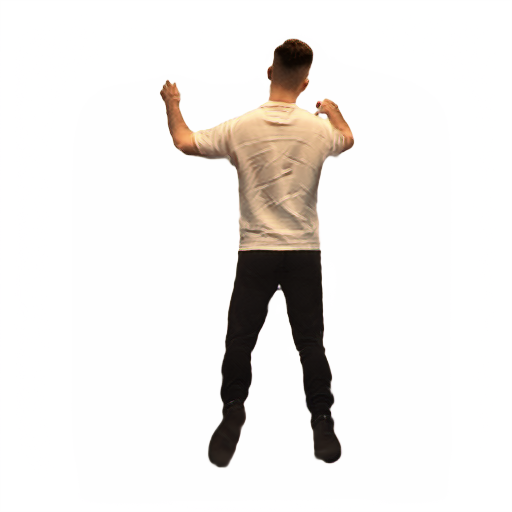
\includegraphics[width=\linewidth]{\imgfp/ntex_patch/fixed}
		\caption{}
		\label{fig:ntex-fixed}
	\end{subfigure}
	\caption{(\protect\subref{fig:ntex-grad}) A mask of non-zero gradients for a neural texture after seeing the whole training sequence. It's common that some body parts are never seen during training, e.g. bottom of shoes, top of the head, armpits. (\protect\subref{fig:ntex-artifact}) Example of rendering instability due to that. (\protect\subref{fig:ntex-fixed}) A crude solution is to replace the unseen parts with a texture part that was actually optimized (e.g. a part of legs or skin). Although it solves the particular artifact on feet, it may not be applicable to the head or armpits.}
\end{figure}
\begin{figure}
	\centering%
	\setlength\abovedisplayskip{0pt}%
	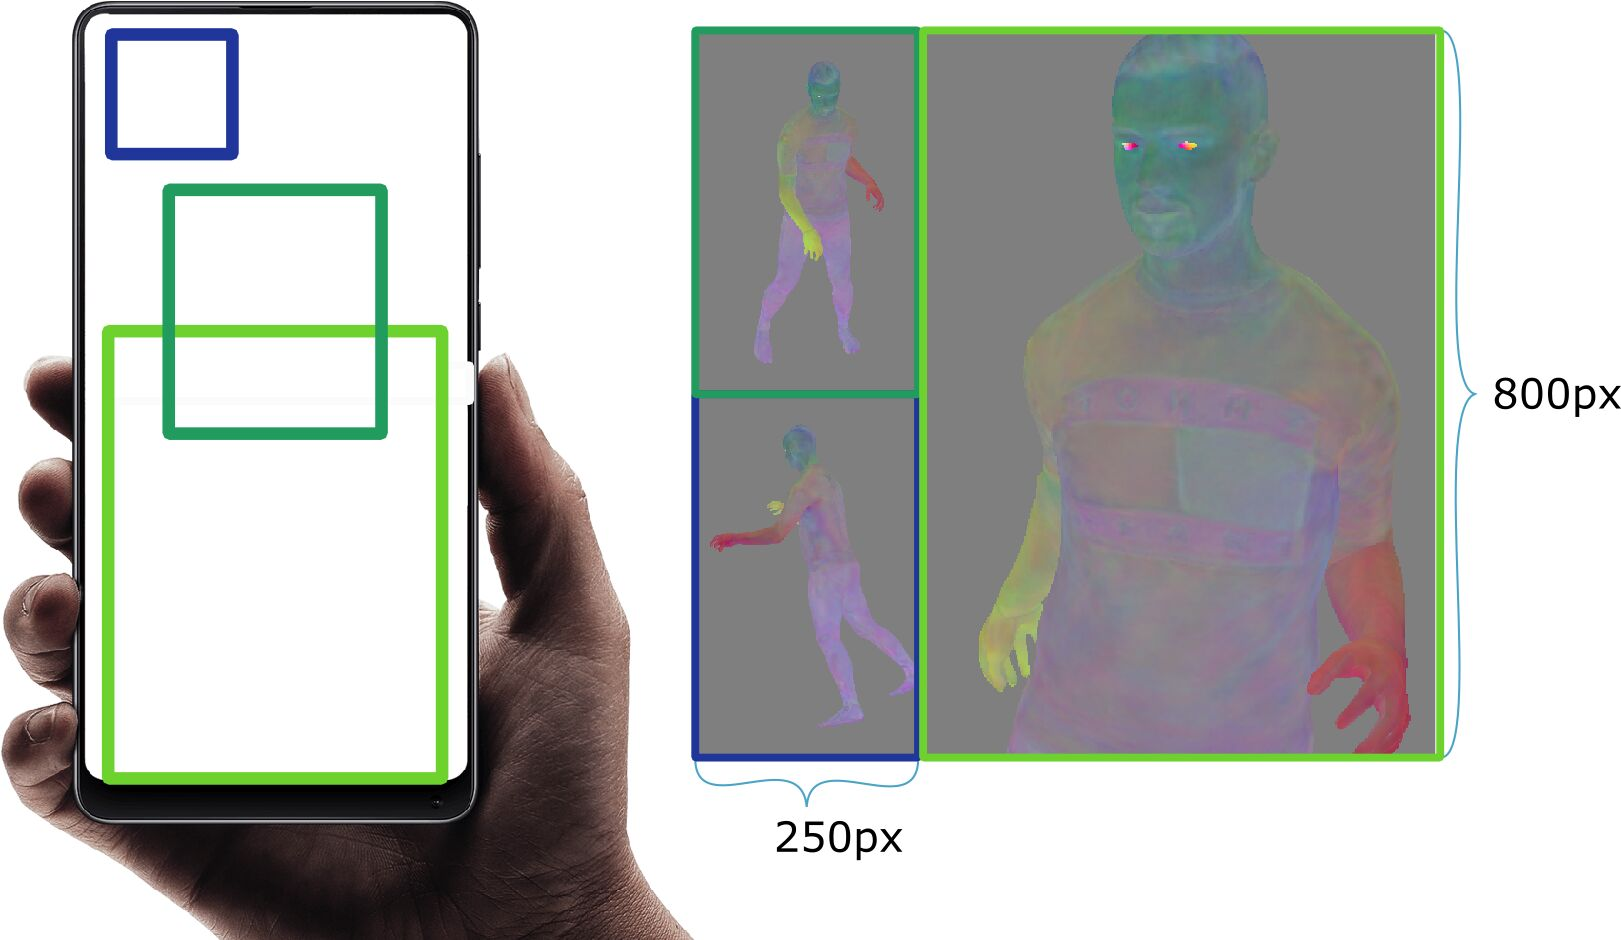
\includegraphics[width=0.6\linewidth]{\imgfp/multiavatar}%
	\caption{Example of a future work on inferring images of multiple avatars. Inputs can be dynamically cropped, rasterized at resolution proportional to occupied space, and collated into a single input tensor. Knowing the screen location of the avatars, the synthesized images can be rendered at proper locations in AR.}%
	\label{fig:multiavatar}%
	\setlength\belowdisplayskip{0pt}%
\end{figure}
\clearpage
\newpage

\section{Mobile application screenshots}
\label{appb:mobile-screenshots}

\begin{figure}[h]
	%\fboxrule=2pt
	\centering
	\begin{subfigure}[b]{0.32\textwidth}
		\centering
		\includegraphics[width=\linewidth]{\imgfp/mobile_inference/A01_07_gpu/000435}%
		\caption{}
		\label{fig:infer_gpu}
	\end{subfigure}
	\hfill
	\begin{subfigure}[b]{0.32\textwidth}
		\centering
		\includegraphics[width=\linewidth]{\imgfp/mobile_inference/A01_07_dsp/000435}
		\caption{}
		\label{fig:infer_dsp}
	\end{subfigure}
	\hfill
	\begin{subfigure}[b]{0.32\textwidth}
		\centering
		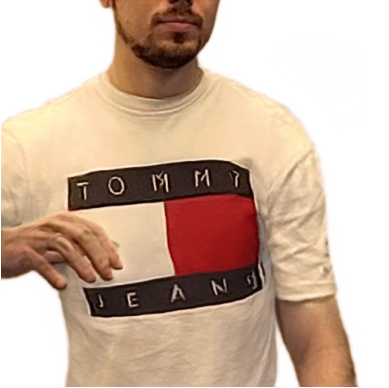
\includegraphics[width=\linewidth]{\imgfp/mobile_inference/A01_07_desktop/mobile_on_desktop35w}
		\caption{}
		\label{fig:infer_desktop}
	\end{subfigure}
	\caption{Comparison of quality loss when synthesizing images on a mobile phone or desktop computer. (\protect\subref{fig:infer_gpu}) was generated on mobile GPU from INT8 quantized input and FP32 weights. (\protect\subref{fig:infer_dsp}) was synthesized on mobile DSP with both input and weights quantized to INT8. It has noticeable discretization noise. (\protect\subref{fig:infer_desktop}) was generated on a desktop GPU using PyTorch with initial FP32 inputs and network weights. The quality is identical to the mobile GPU.}
\end{figure}
\begin{figure}[hb]
	%\fboxrule=2pt
	\centering
%	\begin{subfigure}[b]{0.32\textwidth}
%		\centering
		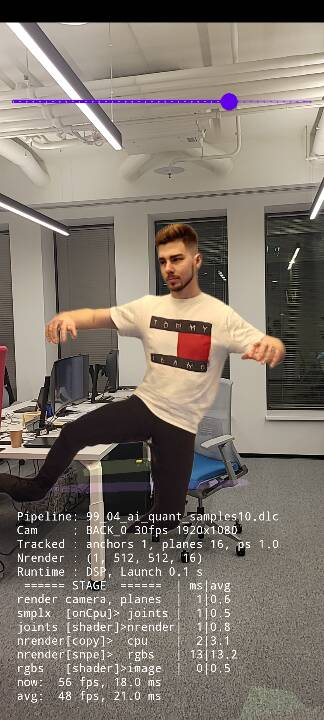
\includegraphics[height=13cm]{\imgfp/mobile_screenshots/jump}%
%		\caption{}
		\label{fig:avatar_jump}
%	\end{subfigure}
%	\hfill
%	\begin{subfigure}[b]{0.32\textwidth}
%		\centering
%		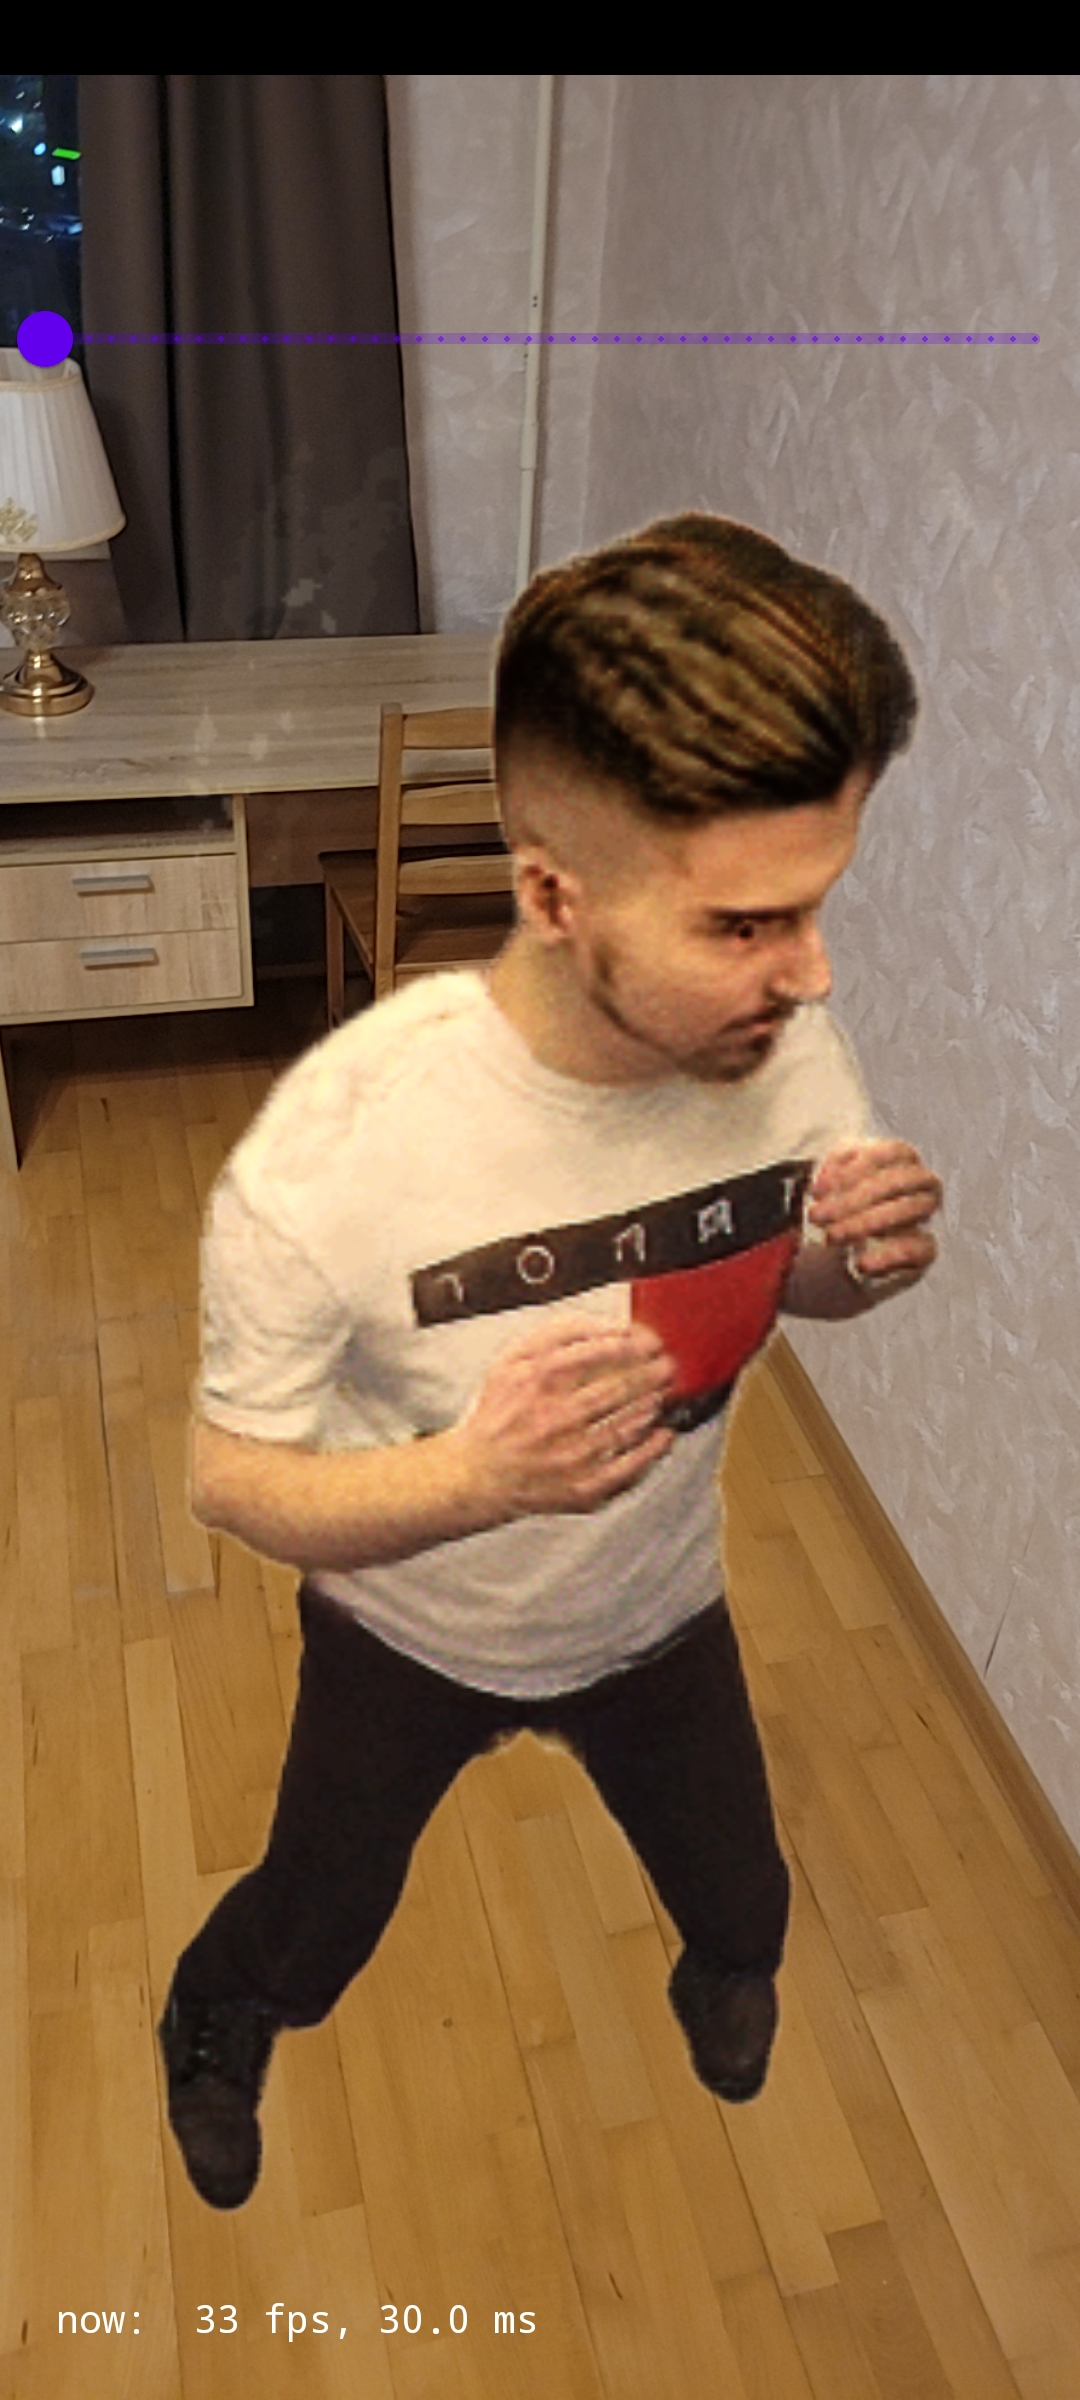
\includegraphics[width=\linewidth]{\imgfp/mobile_screenshots/screen-crop}
%		\caption{}
%		\label{mobile:zoom_screen_crop}
%	\end{subfigure}
%	\hfill
%	\begin{subfigure}[b]{0.32\textwidth}
%		\centering
%		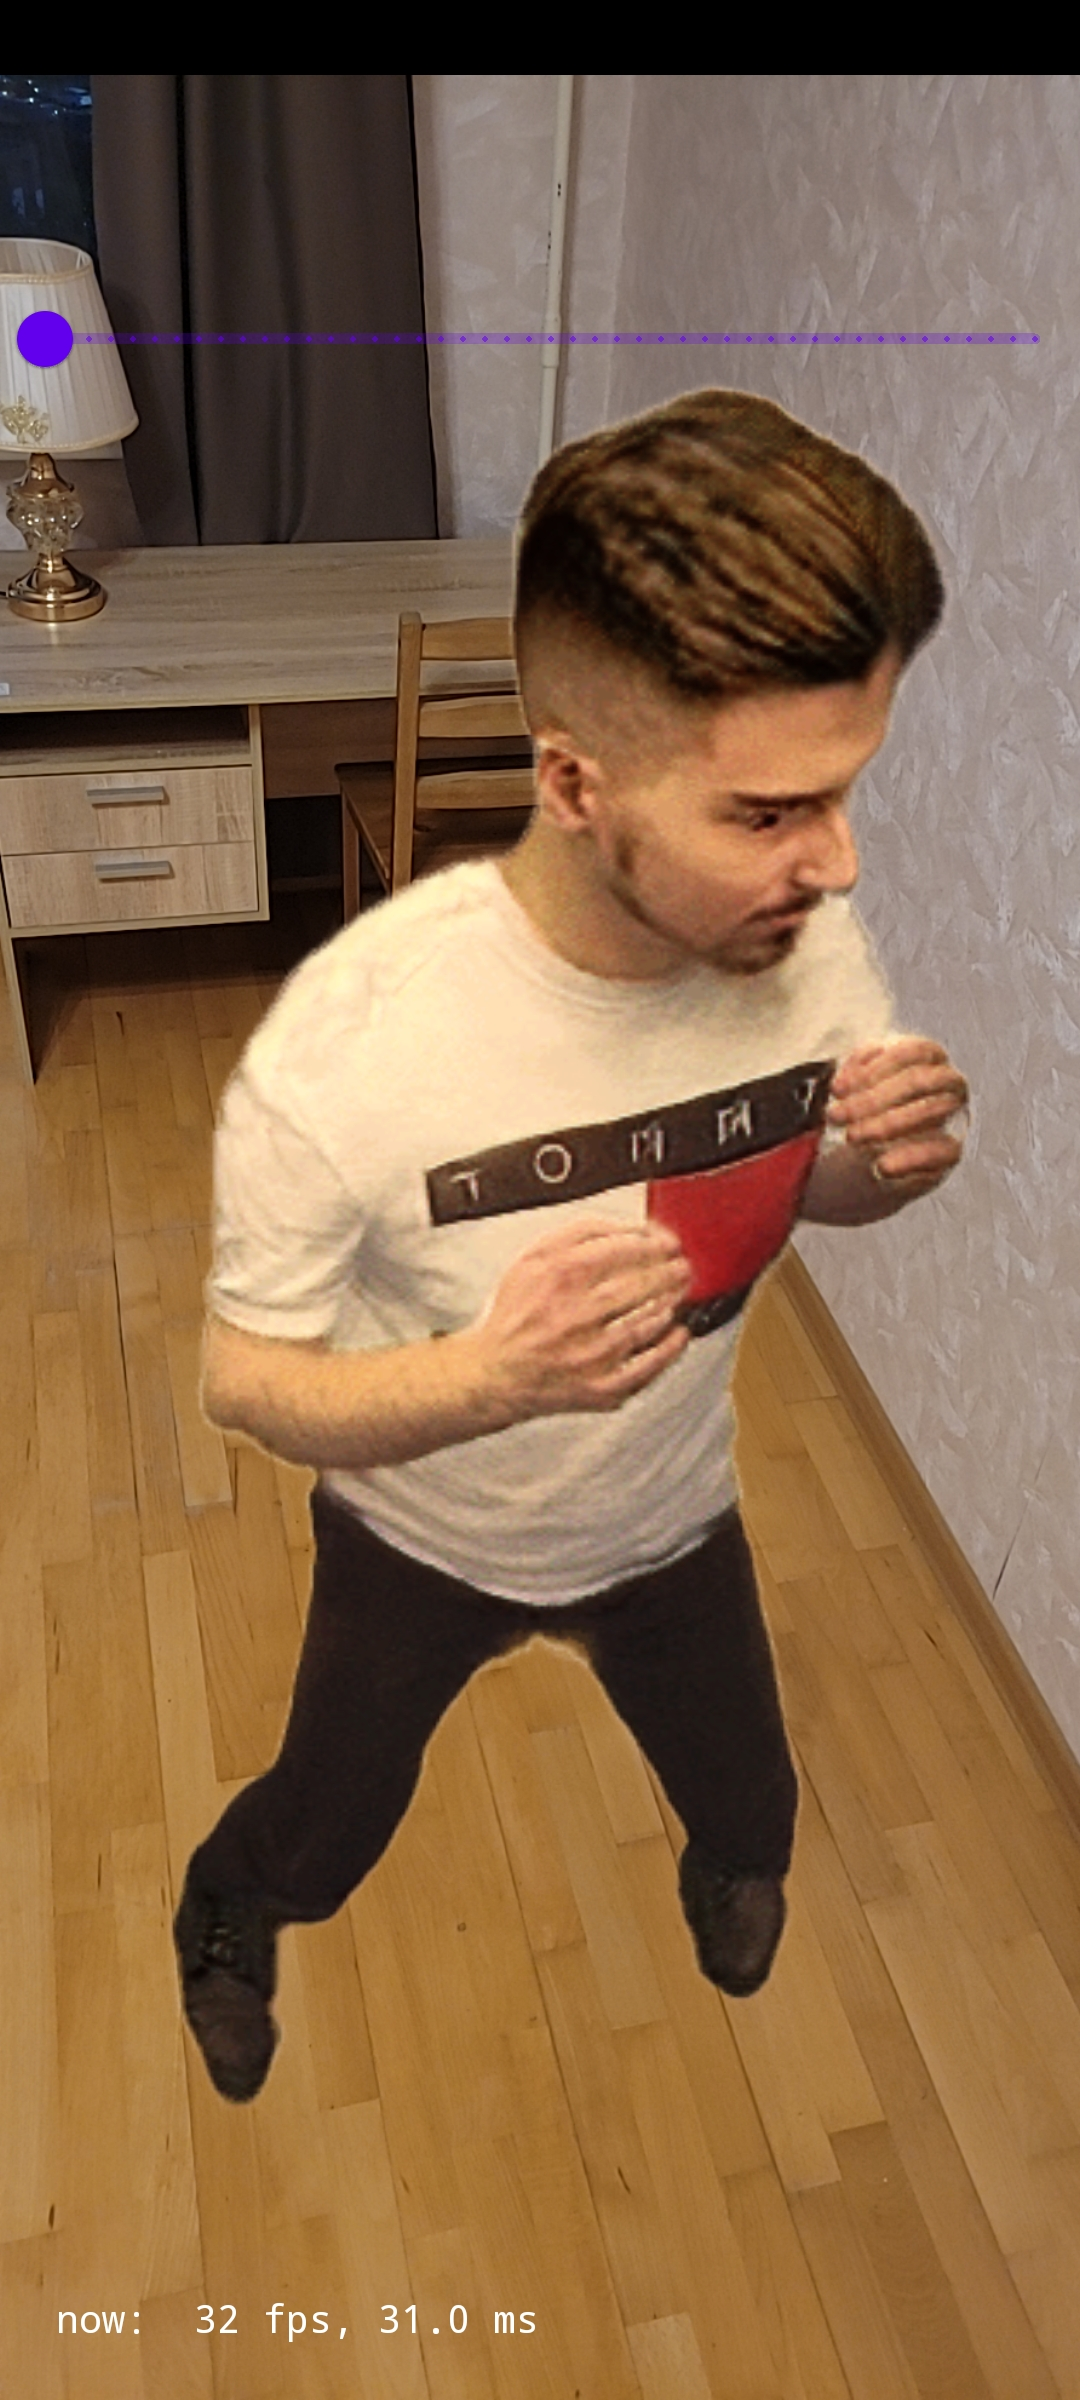
\includegraphics[width=\linewidth]{\imgfp/mobile_screenshots/smallest-crop}
%		\caption{}
%		\label{mobile:zoom_smallest_crop}
%	\end{subfigure}
	\caption{Examples of avatar images in the mobile application. We have predefined animations that can be played with any avatar.}
\end{figure}
\begin{figure}
	%\fboxrule=2pt
	\centering
	\begin{subfigure}[b]{0.32\textwidth}
		\centering
		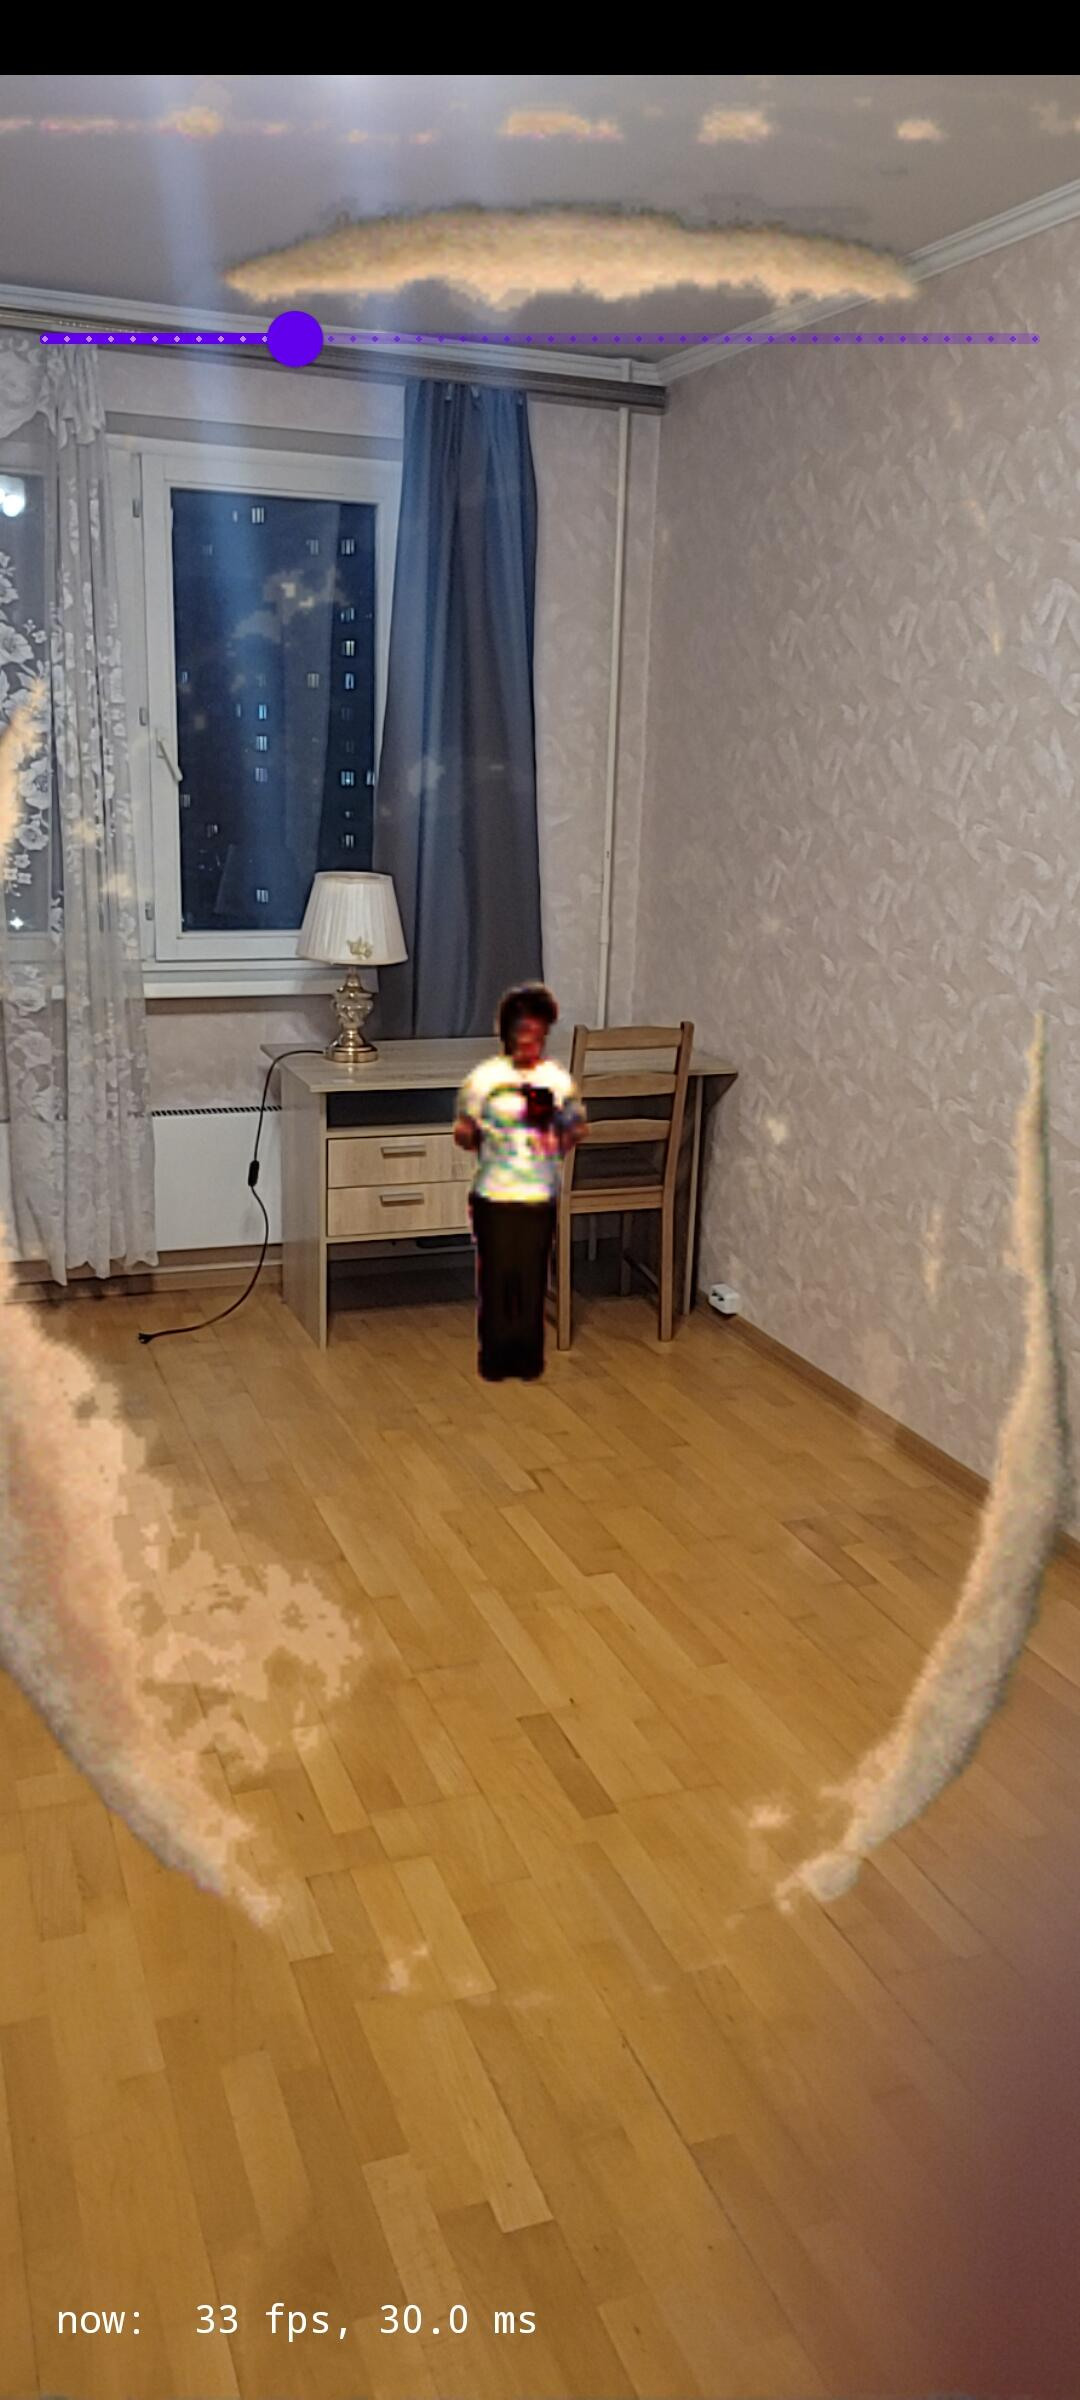
\includegraphics[width=\linewidth]{\imgfp/mobile_screenshots/far-away-screen-crop}%
		\caption{}
		\label{fig:far_screen_crop}
	\end{subfigure}
	\hfill
	\begin{subfigure}[b]{0.32\textwidth}
		\centering
		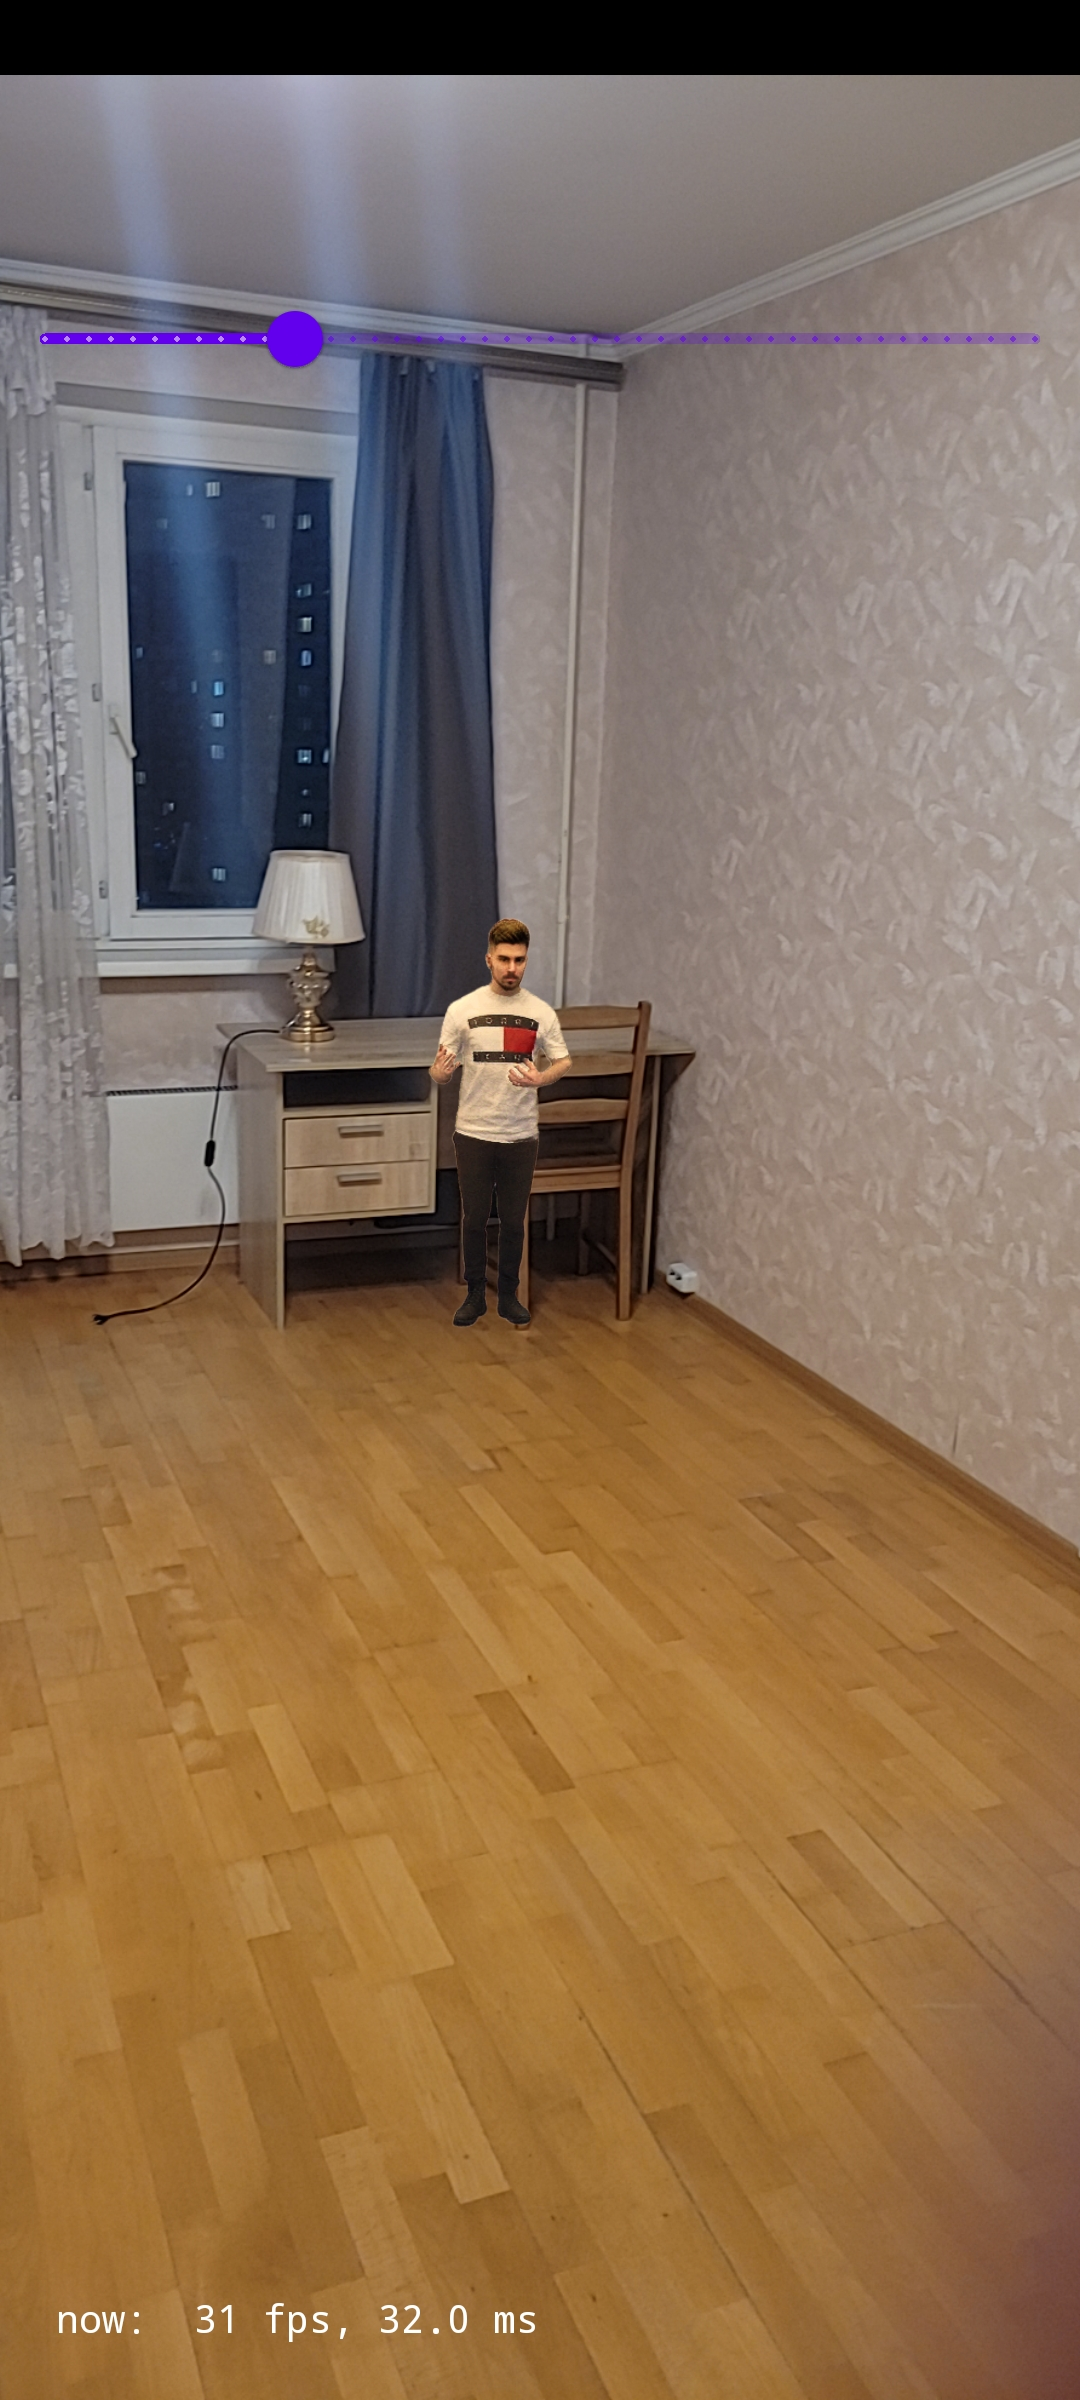
\includegraphics[width=\linewidth]{\imgfp/mobile_screenshots/far-away-crop}
		\caption{}
		\label{fig:far_dynamic_crop}
	\end{subfigure}
	\hfill
	\begin{subfigure}[b]{0.32\textwidth}
		\centering
		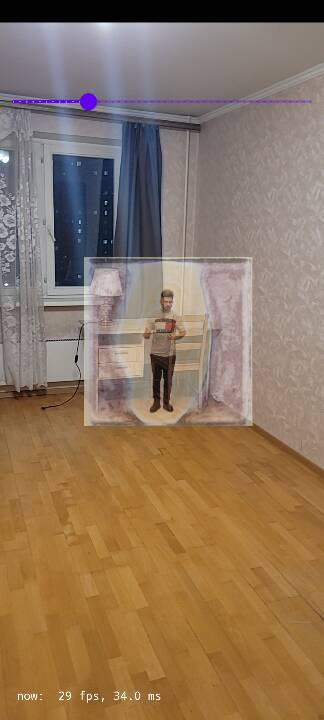
\includegraphics[width=\linewidth]{\imgfp/mobile_screenshots/far-away-crop-debug}
		\caption{}
		\label{fig:far_dynamic_crop_debug}
	\end{subfigure}
	\caption{Comparison of projection modes. (\protect\subref{fig:far_screen_crop}) A projection matrix that spans the whole screen (default mode). Since the input image is square in our pipeline, the input image is effectively much wider than the screen, most of the generated image is wasted. Moreover, the input contains a very tiny rasterization of the mesh, and unless neural network was trained to see such small inputs, it may produce visual artifacts, as shown. (\protect\subref{fig:far_dynamic_crop}) A dynamic crop approach used in this work maximizes the avatar in the input rasterization, thus the network produces an image of sufficient quality. (\protect\subref{fig:far_dynamic_crop_debug}) Shows the output image without segmentation mask applied, allowing to see the borders of the dynamic crop. It covers all the joints and expands or shrinks on every frame.}
\end{figure}
\begin{figure}
	%\fboxrule=2pt
	\centering
	\begin{subfigure}[b]{0.32\textwidth}
		\centering
		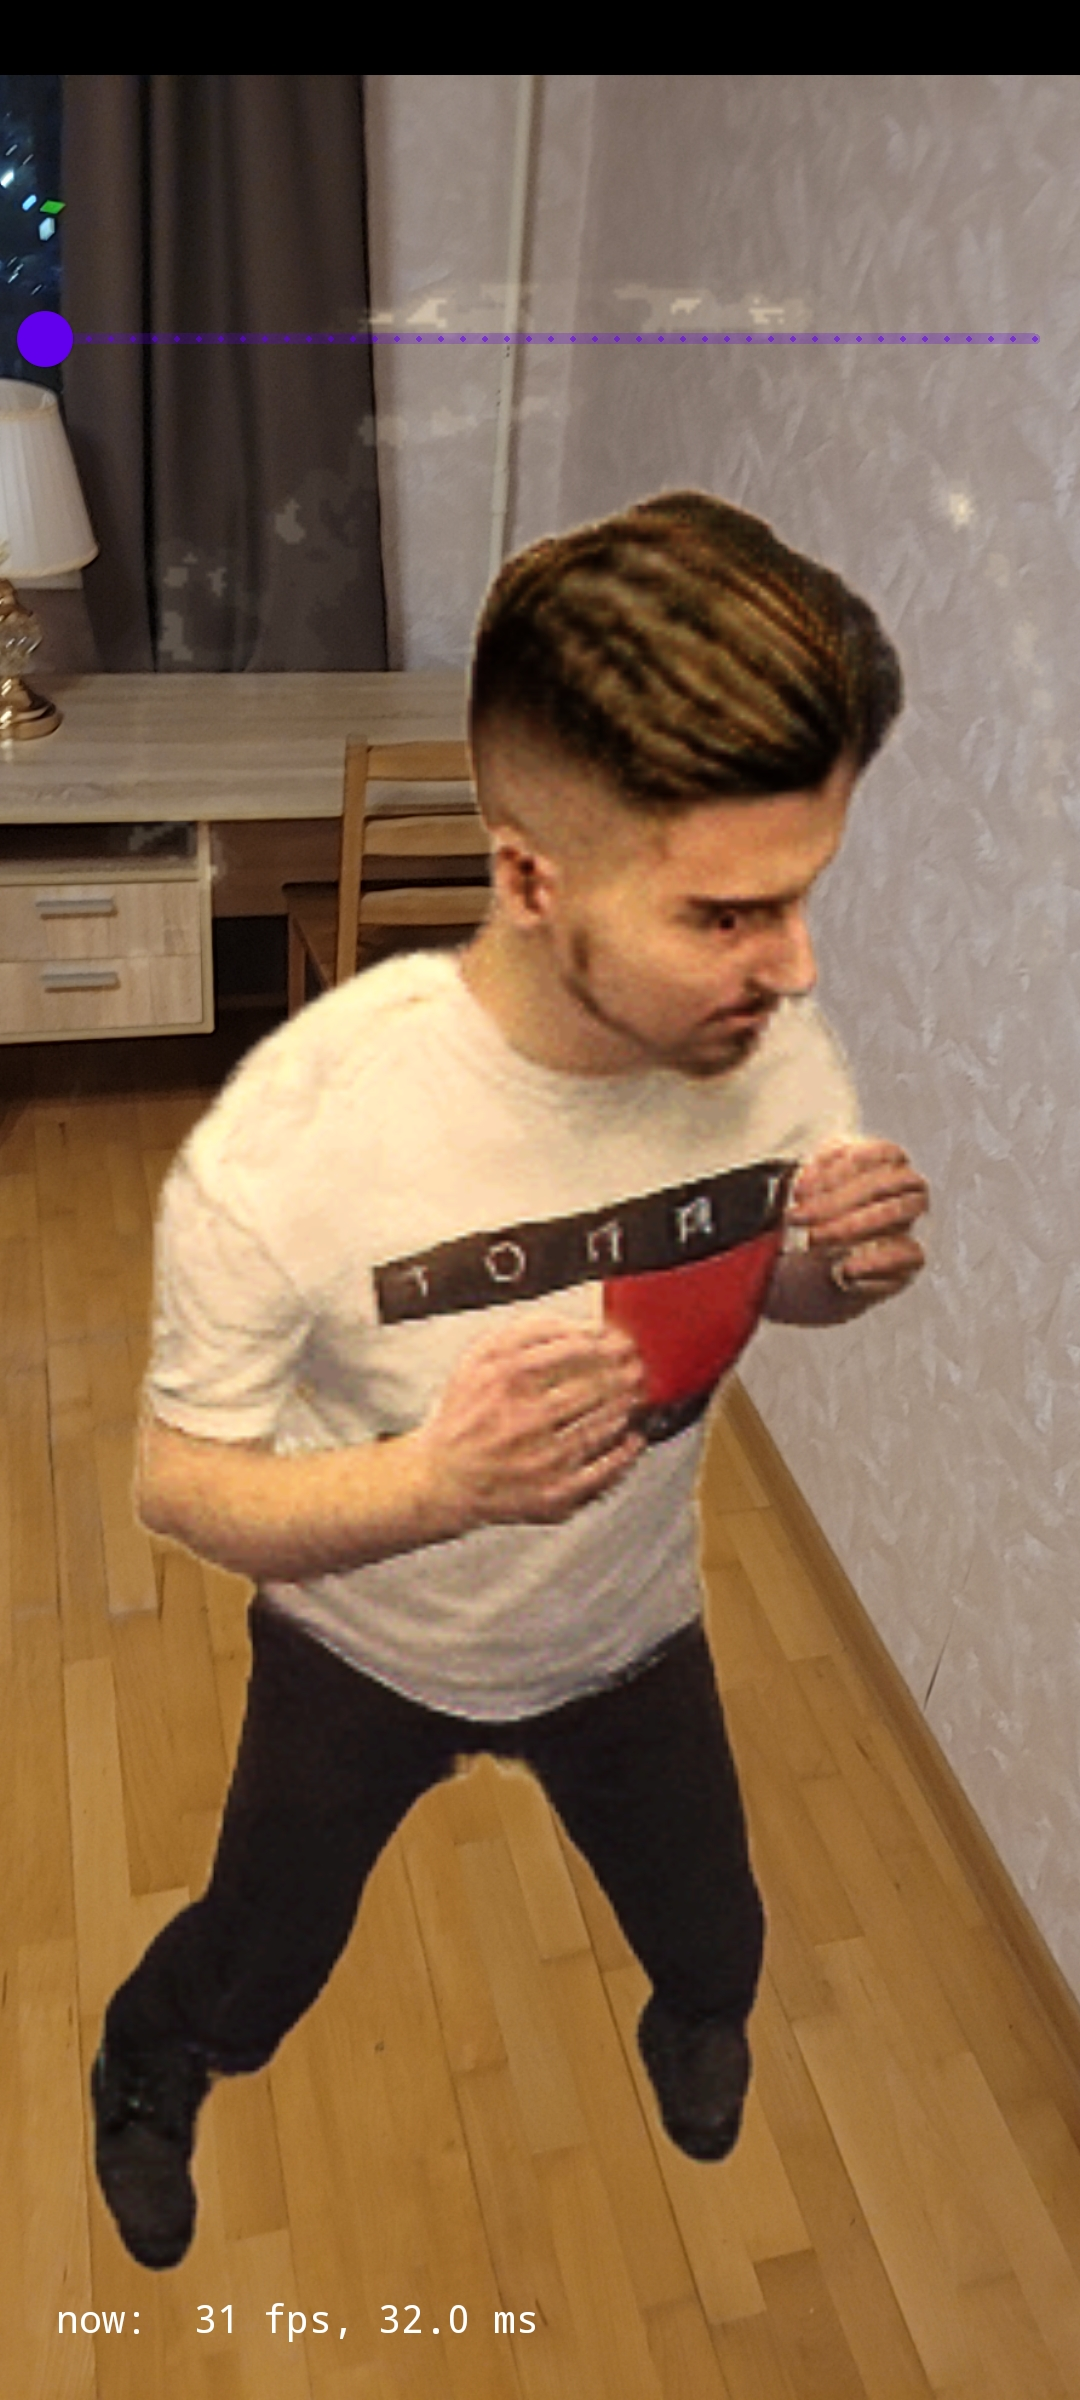
\includegraphics[width=\linewidth]{\imgfp/mobile_screenshots/inefficient-crop}%
		\caption{}
		\label{fig:zoom_inefficient_crop}
	\end{subfigure}
	\hfill
	\begin{subfigure}[b]{0.32\textwidth}
		\centering
		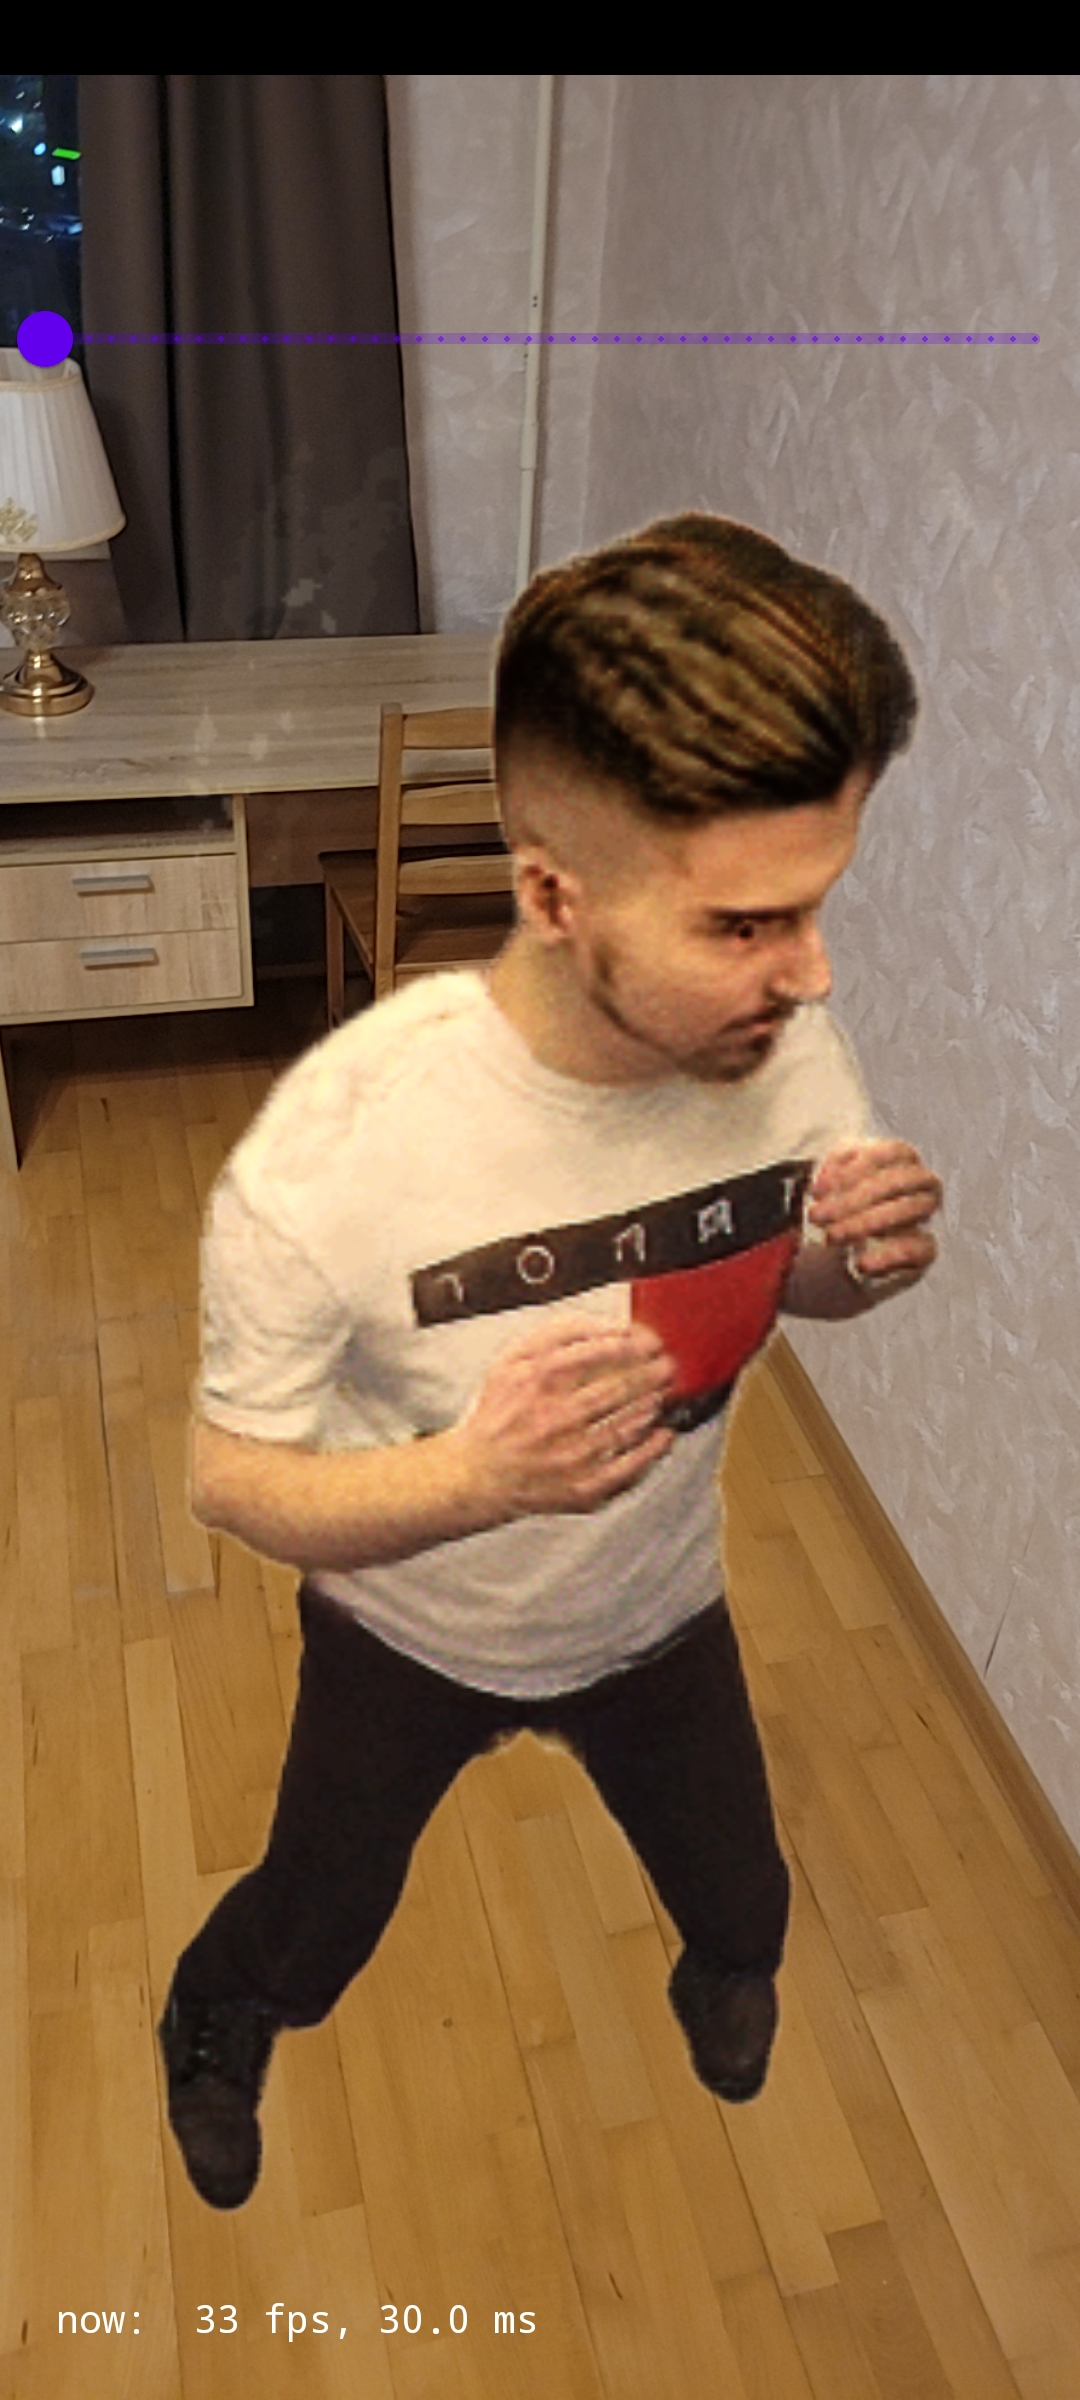
\includegraphics[width=\linewidth]{\imgfp/mobile_screenshots/screen-crop}
		\caption{}
		\label{fig:zoom_screen_crop}
	\end{subfigure}
	\hfill
	\begin{subfigure}[b]{0.32\textwidth}
		\centering
		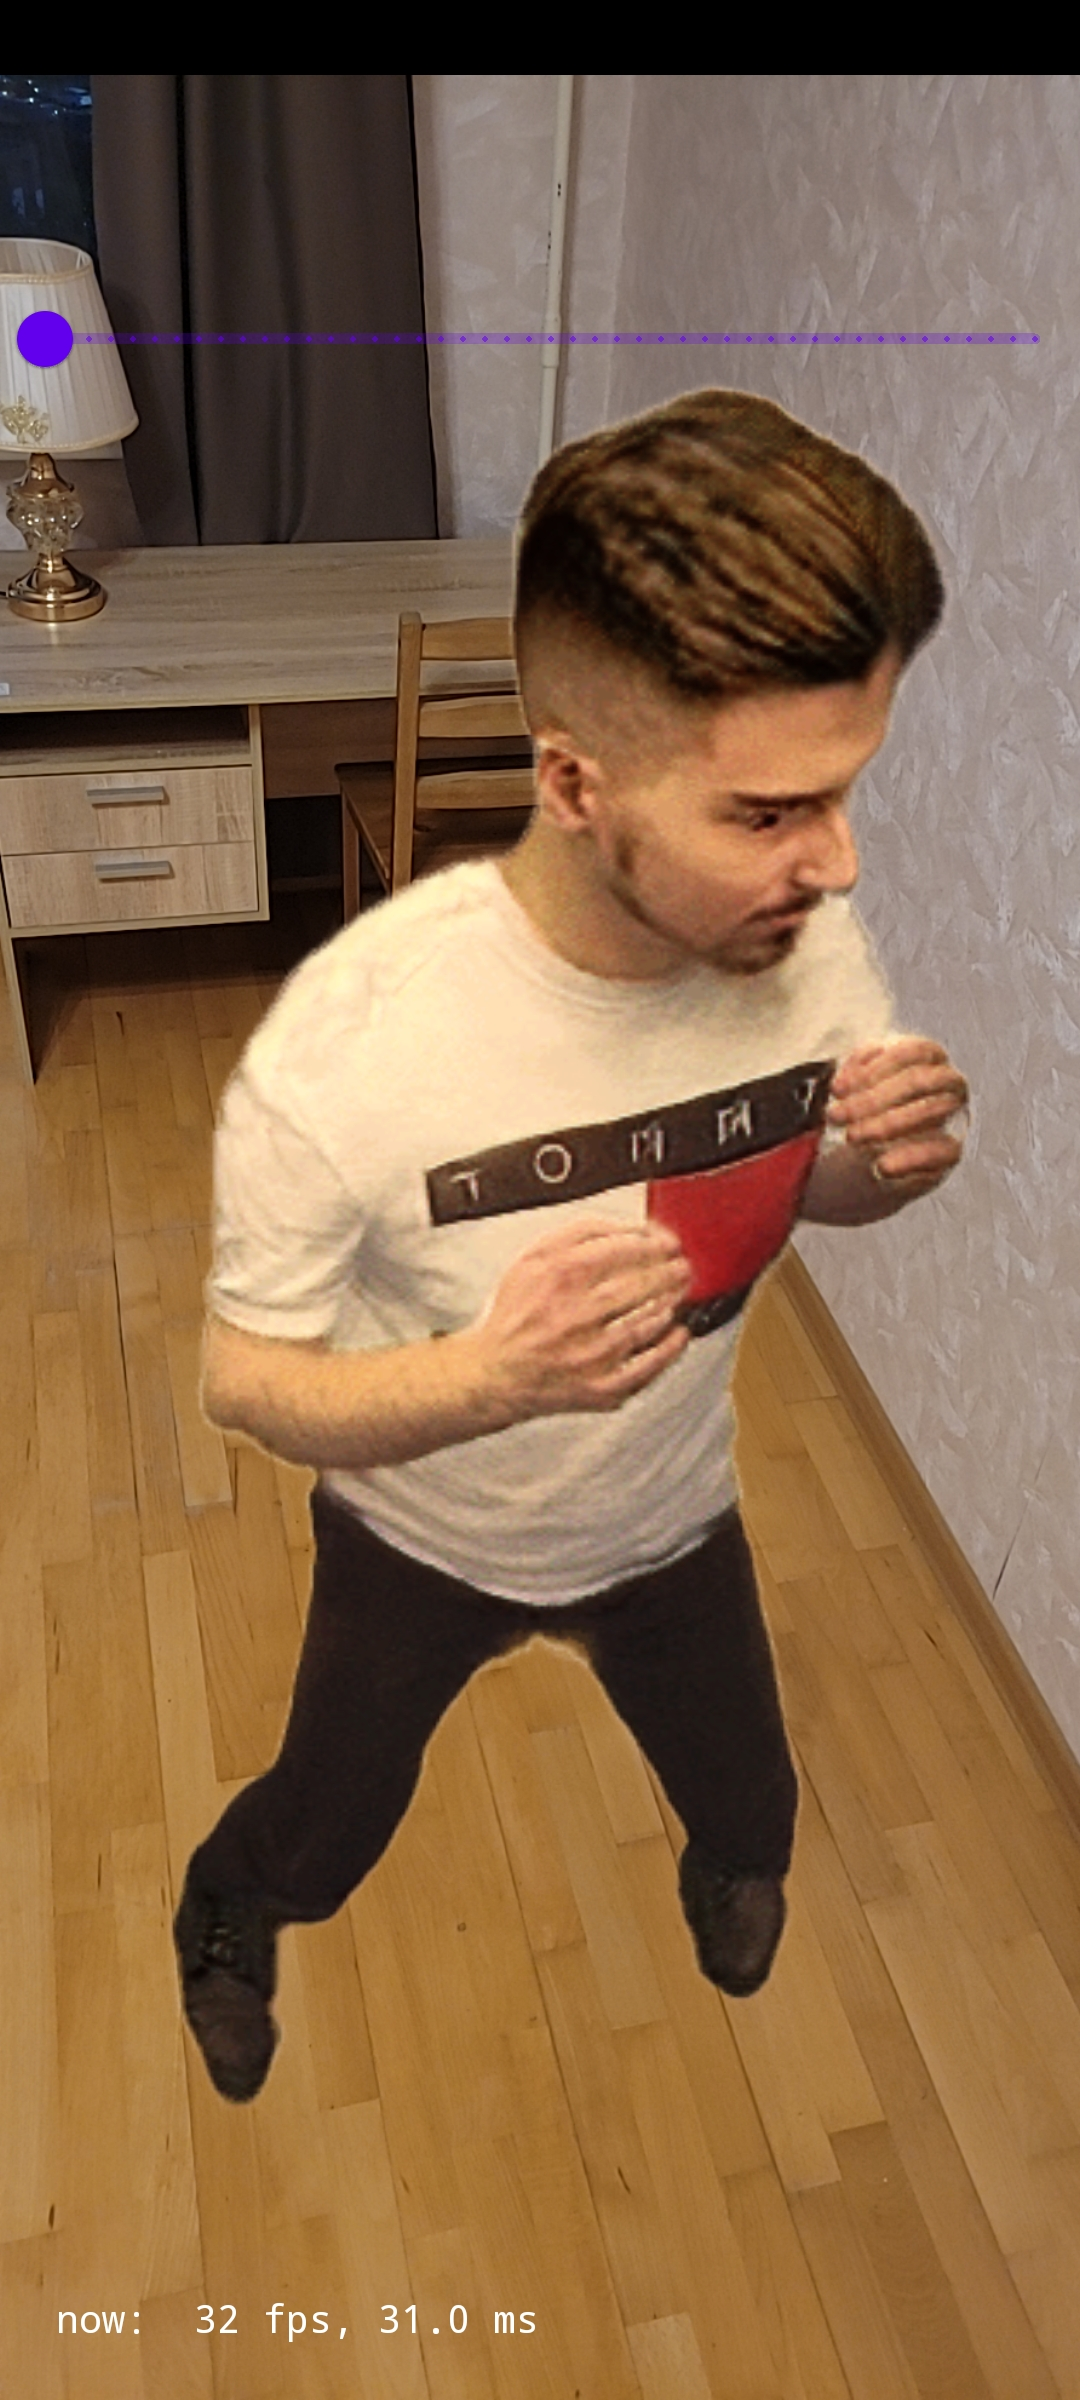
\includegraphics[width=\linewidth]{\imgfp/mobile_screenshots/smallest-crop}
		\caption{}
		\label{fig:zoom_smallest_crop}
	\end{subfigure}
	\caption{Comparison of projection modes in close view. (\protect\subref{mobile:zoom_inefficient_crop}) A projection matrix that spans the whole screen (default mode). Even if the avatar spans almost all the screen, parts of the frame are still being wasted, decreasing possible resolution of the avatar. Some artifacts appear, similarly to what shown on Figure \ref{mobile:far_screen_crop}. (\protect\subref{mobile:zoom_screen_crop}) A dynamic crop around all the joints. A bit higher quality in this scenario, but the crop is similar to full-screen projection. (\protect\subref{fig:zoom_smallest_crop}) A dynamic crop around only seen body parts. Yields the highest quality, since it minimizes the area of wasted space.}
\end{figure}
\clearpage
\newpage

\section{Training procedure experiments}
\label{appb:exps}
Next we demonstrate most of the experiments as collations of training and test images, as well as plots of training losses and plots of validation metrics. Images encased with a gray border are \textit{synthesized}, the border-less images are ground truth. Each column of the images has a colored mark at the bottom. It represents a corresponding line color on the plots for the given experiment. The legends of the plots contain a short description of the experimental setup and adjustments. To shorten the descriptions, we use a notation like $\Omega=$ to show that any other usage of $\Omega$ on the same plot uses or extends from this experiment. 

To keep this section compact, we demonstrate only a subset of loss and metric curves, namely LPIPS, L1, MS-SSIM, and adversarial losses. A single plot of the adversarial loss will combine two lines: generator's loss (solid line) is accuracy of the discriminator on the synthesized images, the discriminator's loss (translucent line with colored dots) is accuracy of the discriminator on the real images. The former should decrease, indicating that the generator produces plausible images, and the latter should increase, indicating that the discriminator learns the realism of ground truth images.

As a minimal subset of training images, we show full-body and upper body frames with the most difficult poses available, frames from front and back, as well as a close-up shot of a face. The selected test frames contain:
\begin{itemize}
	\item Bottom of the shoes -- showing artifacts for the body parts that were unseen during training.
	\item A face close-up -- may lose similarity with the person's face due to overfitting.
	\item A top-down view, which may show overfitting to the frames in the training set, where the person bends forward, and a shadow is cast upon their upper body (see training images, first row). Even though the test pose is different, the overfitting triggers the same shadow to appear on the synthesized image.
	\item An upper-body, to compare clarity of T-shirt ornaments, which may be lost due to possible misalignment of the ground truth images and the body model \cite{dnn:smplx19}. Thus, the pixels of the neural texture may fit different locations on the body.
	\item A front full-body view, to compare overall body quality.
\end{itemize}

\newcounter{experiments-group}
\setcounter{experiments-group}{1}

\setkeys{Gin}{draft}
\clearpage
\newpage
\arabic{experiments-group}. \alert{Experiments on neural texture's MIP-maps (no Omega definition for test plot)}
\stepcounter{experiments-group}
%\begin{adjustwidth}{-20em}{-8em}

% convert -strip -interlace Plane -quality 95% -adaptive-resize 85% TEST_05_54_r1\@vA01_41\@vA01_41_learnmips\@vA01_41_nomips.png out2.jpg
\begin{figure}[!h]
	\makebox[\textwidth]{\makebox[1.1\textwidth]{
	\begin{minipage}[b]{.59\textwidth}
		\centering%
		\setlength\abovedisplayskip{0pt}%
		\centerline{\includegraphics[width=1.0\textwidth]{\imgfp/exp_train/TRAIN_05_54_r1@vA01_41@vA01_41_learnmips@vA01_41_nomips}}%
		\caption{Fit to ground truth}
		\setlength\belowdisplayskip{0pt}%
	\end{minipage}\hfill
	\begin{minipage}[b]{.50\textwidth}
		\centering%
		\setlength\abovedisplayskip{0pt}%
		\centerline{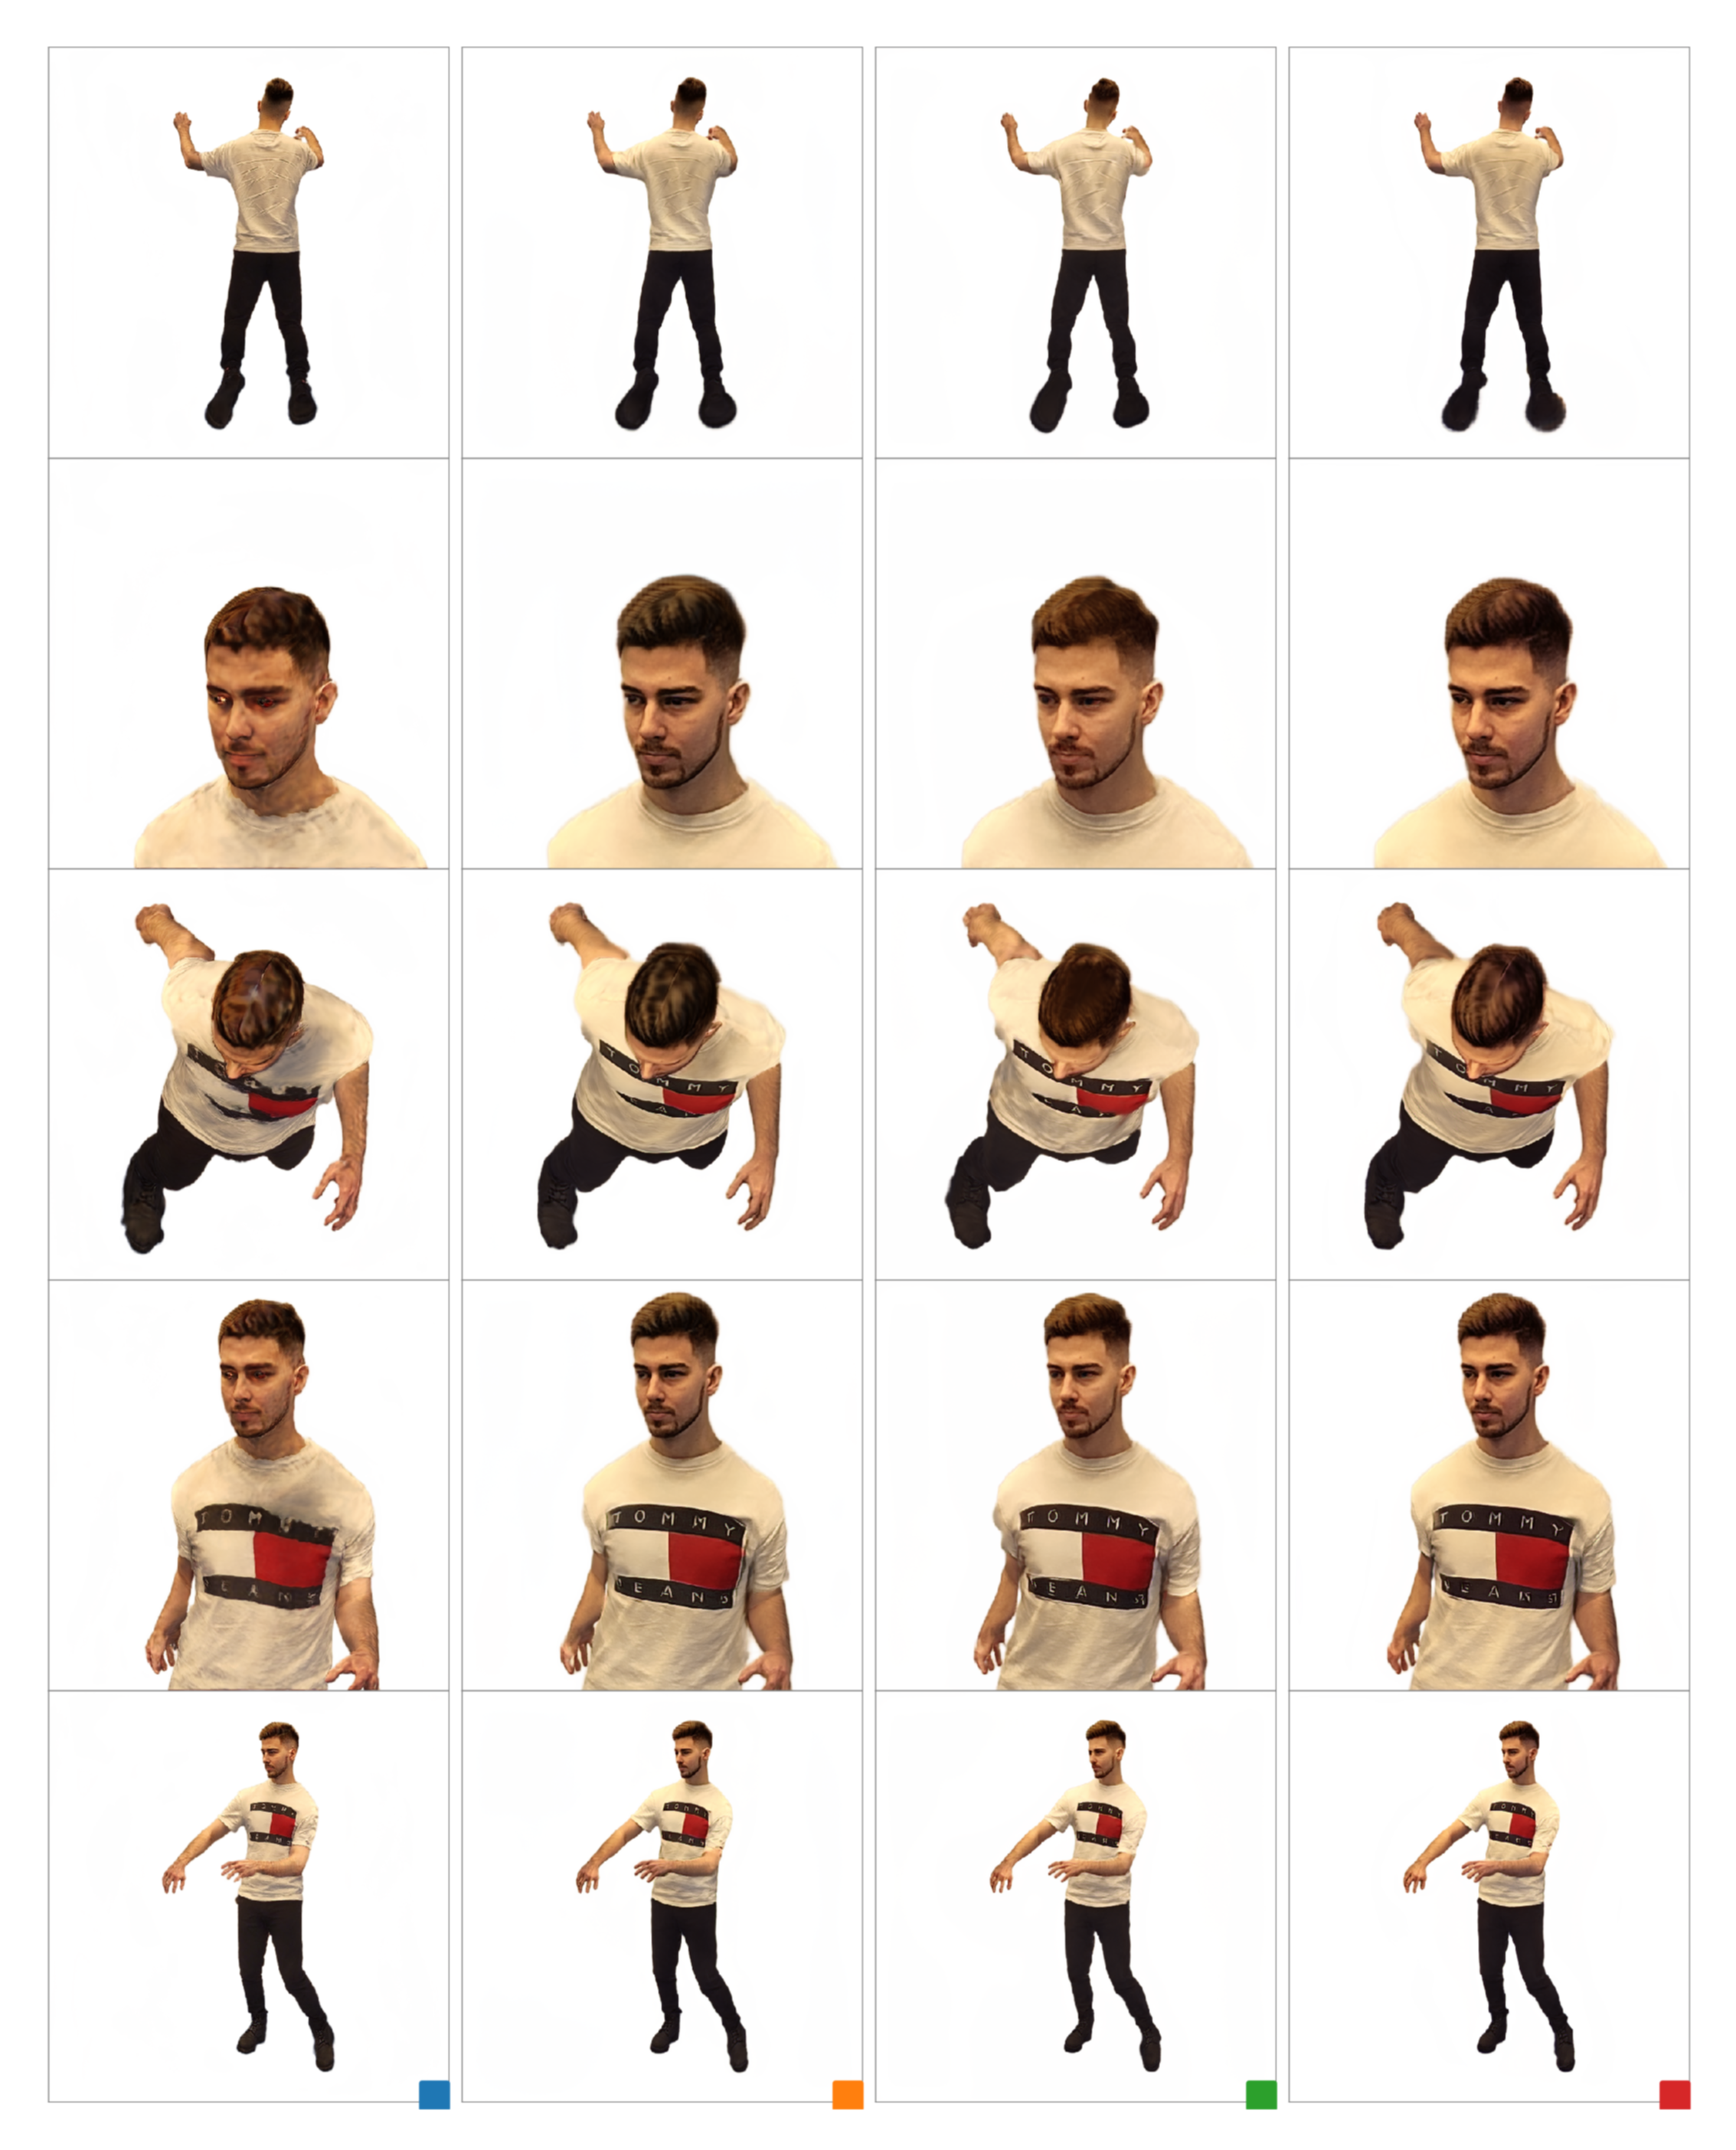
\includegraphics[width=1.0\textwidth]{\imgfp/exp_test/TEST_05_54_r1@vA01_41@vA01_41_learnmips@vA01_41_nomips}}%
		\caption{Test images}
		\setlength\belowdisplayskip{0pt}%
	\end{minipage}
	}}
	\centering%
	%\hspace{.1\textwidth}%
	\setlength\abovedisplayskip{0pt}%
	\centerline{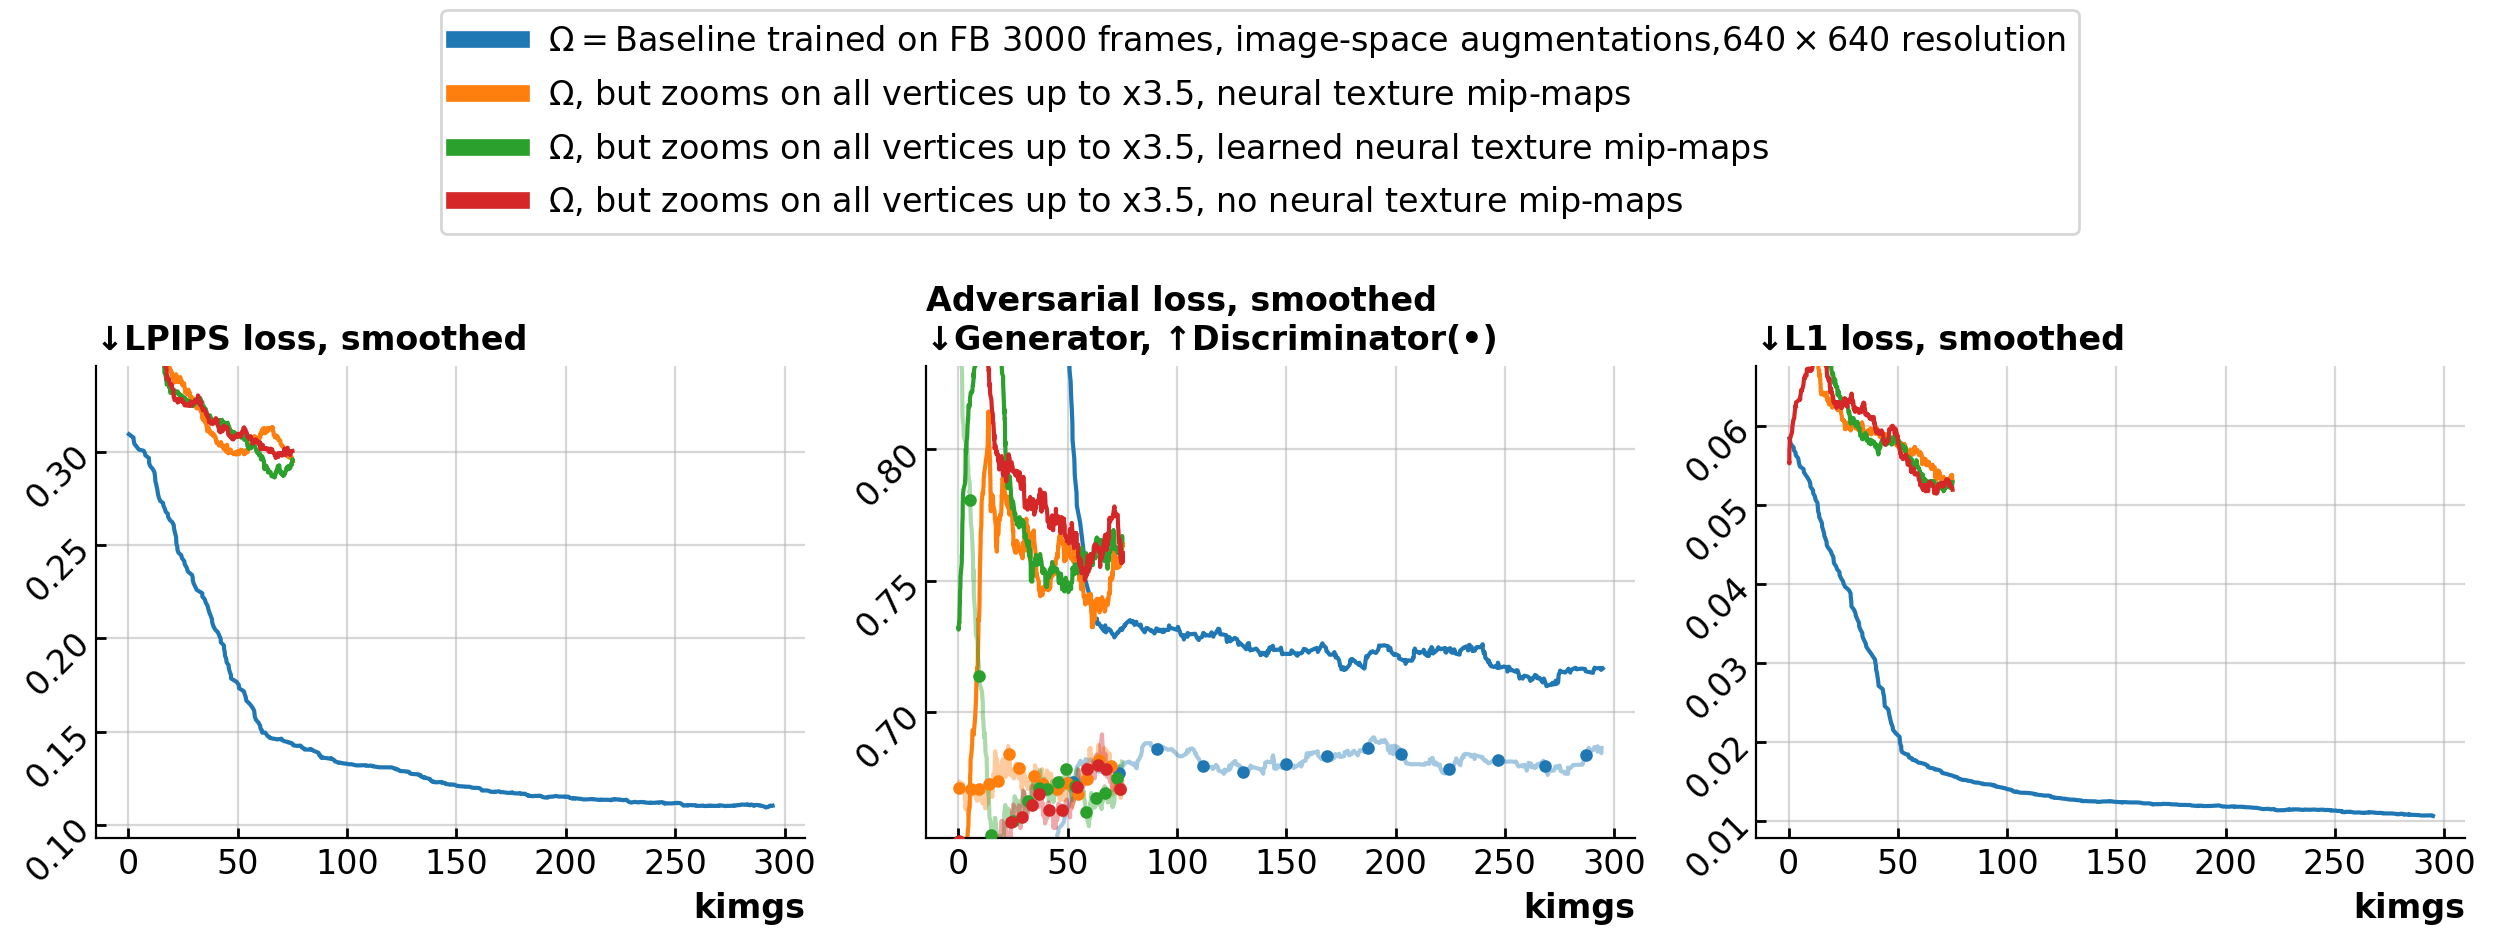
\includegraphics[width=0.99\linewidth]{\imgfp/exp_train/train_plot_05_54_r1@vA01_41@vA01_41_learnmips@vA01_41_nomips}}%
	\hspace{.1\textwidth}
	\centerline{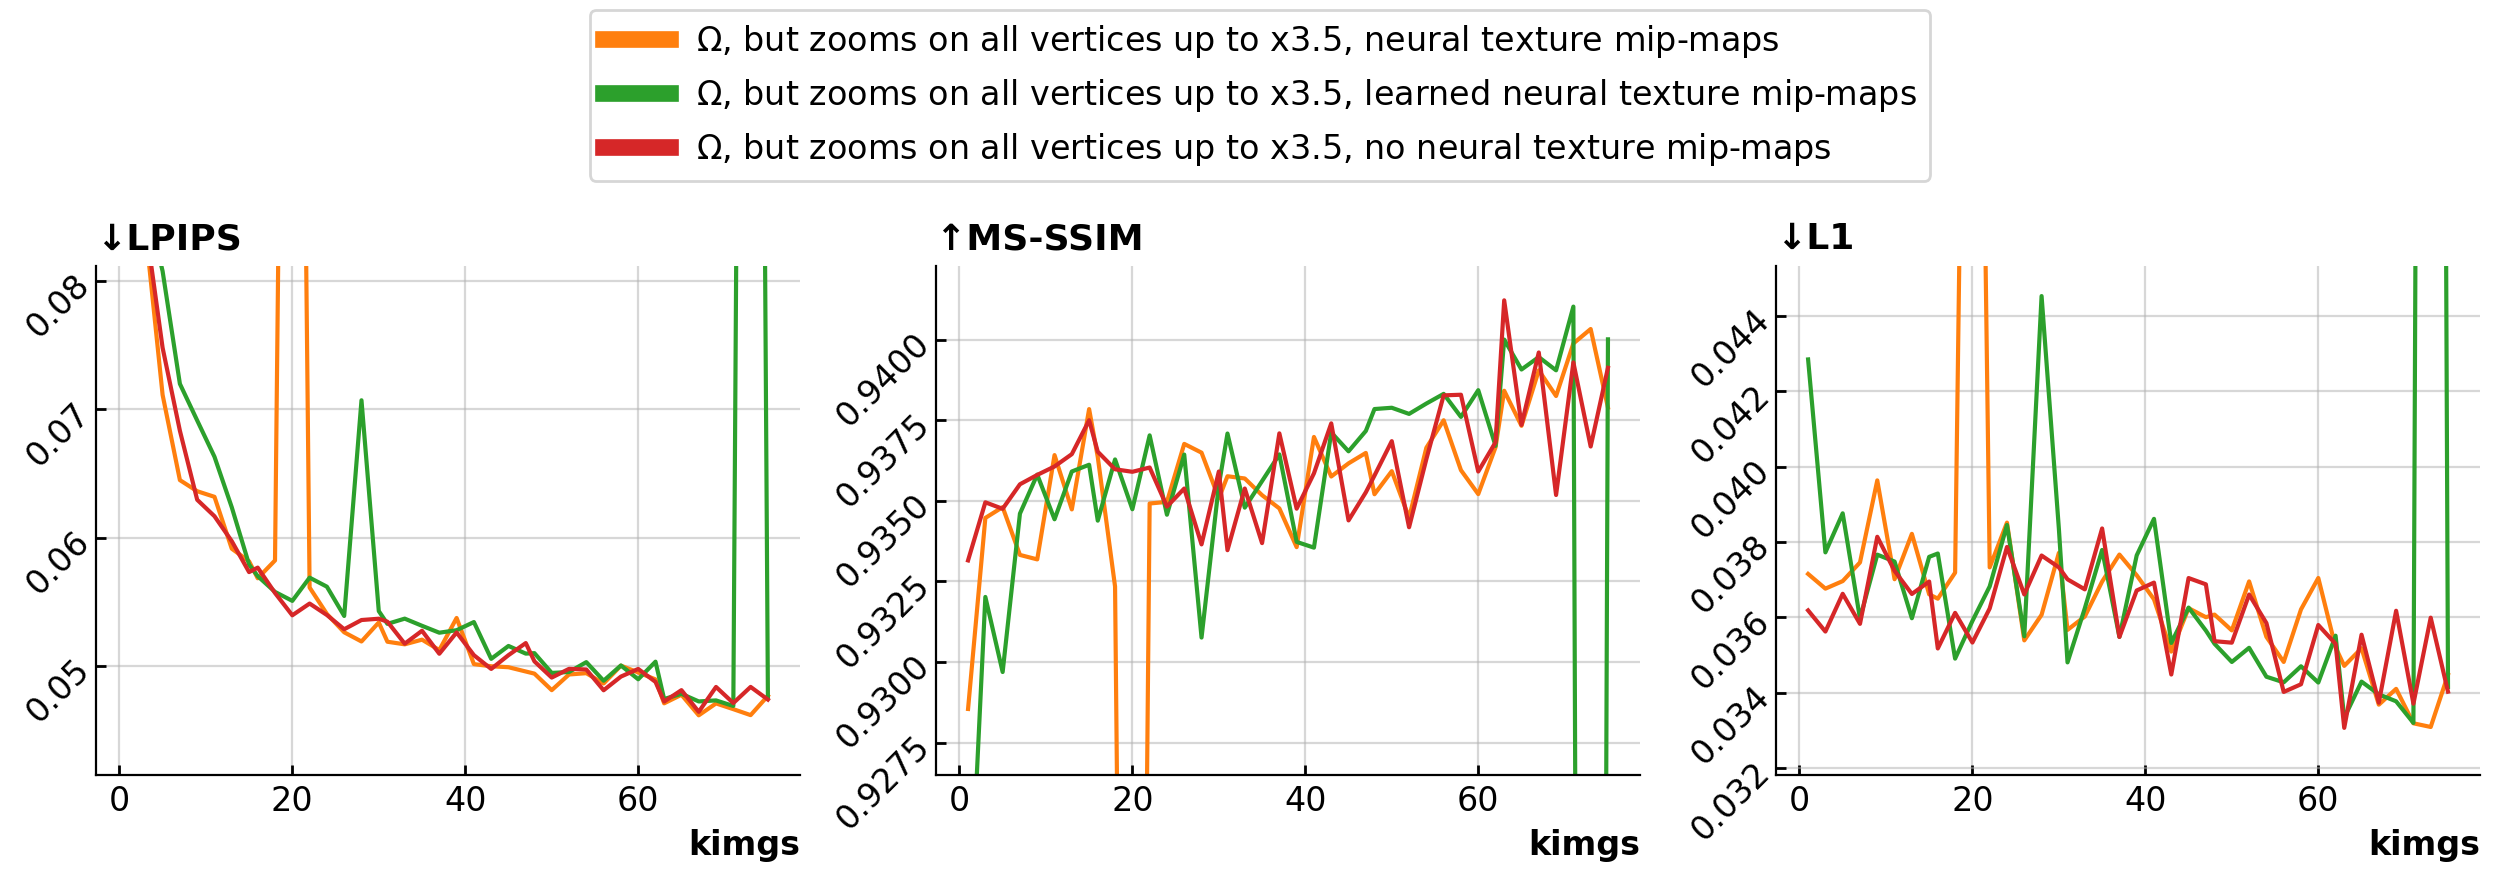
\includegraphics[width=0.99\linewidth]{\imgfp/exp_test/val_plot_05_54_r1@vA01_41@vA01_41_learnmips@vA01_41_nomips}}%
	\setlength\belowdisplayskip{0pt}%
	\caption{Training losses and validation metrics}
\end{figure}
%\end{adjustwidth}

\newpage


\setkeys{Gin}{draft=false}
